%Resultados experimentales
\chapter{Maniobras Cooperativas}\label{sec:capitulo6}
\thispagestyle{empty}

En el presente capítulo se describen las maniobras coperativas realizadas, ACC, Control Lateral, \textit{Stop and Go} y ACC con Control Lateral. Explicando para las dos primeras maiobras, el algoritmo de control realizado, así como su implementación en Dynacar, ambos basados en la lógica difusa.\\

\par Posteriormente se describen las pruebas realizadas, así como sus resultados, teniendo para el ACC y el \textit{Stop and Go}, pruebas de desempeño a bajas y medias velocidades, y para el Control Lateral, tanto con el ACC, como sin el mismo, pruebas con distintos tipos de curvas, más específicamente las presentadas en el escenerio de TECNALIA \textit{Research \& Innovation}.  


\section{ACC Longitudinal}
Como se expuso anteriormente , esta maniobra busca mantener la velocidad del vehículo, tomando en cuenta la velocidad del carro que tiene al frente, así como guardar cierta distancia con respecto al mismo. Para conseguir esto, se realizó un controlador difuso\cite{perez2013cooperative} que recibe como entradas los errores de velocidad y de distancia, y como salida, las respectivas acciones sobre los actuadores.  

\subsection{Algoritmo de Control}

Para comprender mejor las consideraciones empleadas para desarrollar el algoritmo, se presenta la Figura \ref{fig:acce}, en donde, se tienen tres distancias, $ D_{L-S}$, $ D_{S}$ y D. Siendo $D_{L-S}$ la distancia actual entre los vehículos, $D_{S}$ la distancia de seguridad establecida, que a efectos del presente trabajo posee un valor de 7 m, y finalmente D, la distancia ideal a la cual deberían de estar los vehículos.\\

\begin{figure}[!h]
	\centering
		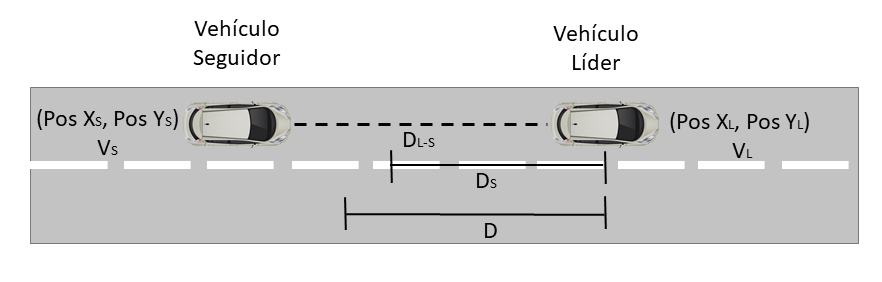
\includegraphics[scale=0.5]{Imagenes/acce}
		\caption{Caractrísticas del ACC implementado}
		\label{fig:acce}
	\end{figure}	 

\par Entonces, teniendo en cuenta que se trabaja con la velocidad y la posción X y Y, de los vehículos, los errores son calculados de la siguiente forma:

\begin{itemize}
\item Error de Velocidad: para el cálculo del error de velocidad, basta con solo la resta de las mismas.
\begin{equation} \label{eq: errvel}
E_{Vel} = V_{L} - V_{S}
\end{equation}
\par Error, que si resulta positivo, quiere decir que la velocidad del vehículo líder es mayor a la del seguidor, por ende el carro seguidor deberá acelerar, mientras que si es negativo la velocidad del vehículo seguidor es mayor a la del líder, por lo que el carro deberá frenar. Siempre y cuando la distancia entre los vehículos no sea muy grande, caso en el cual el vehículo seguidor deberá acelerar para alcanzarlo sin importar la velocidad del vahículo líder.
\item Error de Distancia: para calcular este error se restan los valores de $D_{L-S}$ y D, los cuales se obtienen de la siguiente forma:
\begin{itemize}
\item Distancia entre vehículos: como se poseen son los valores de la posciión X, Y de los carros, se procede a buscar la distancia entre dos puntos.
\begin{equation} \label{eq: distv}
D_{L-S} = \sqrt{(X_{L}-X_{S})^{2} + (Y_{L}-Y_{S})^{2}}
\end{equation}

\item Distancia de referencia: para calcular esta distancia, se hizo uso de la fórmula del cuadrado de la velocidad, dada por la dirección general de tráfico española, DGT \footnote{http://www.dgt.es/es/seguridad-vial/}, a la cual por razones de seguridad se le añadieron 7 m más, que corresponden a la distancia de seguridad. 

\begin{equation} \label{eq: diss}
D = (Entero(\frac{V_{S}}{10}))^{2} + D_{S}
\end{equation}

\end{itemize}
\par Con lo cual error de la distancia resulta:
\begin{equation} \label{eq: errvel}
E_{Dist} = D_{L-S} - D
\end{equation}

\par Valor que si da positivo quiere decir que se supera la distancia de referencia, implicando que el vehículo deberá de acelerar, mientras que si es negativo, la distancia entre los vehículos es menor que la de referencia, por lo que el carro tendrá que frenar.

\end{itemize} 
\subsection{Implementación en el Simulador}

Para la implementación en Dynacar de este controlador se hizo uso del ToolBox de MATLAB para controladores difusos, al cual se le pasan como entradas las variables medidas, que en este caso son el error de la velocidad y el error de la distancia, y como salida las variables a controlar, acelerador y freno (Figura \ref{fig:accdyna})\\ 

\begin{figure}[!h]
	\centering
		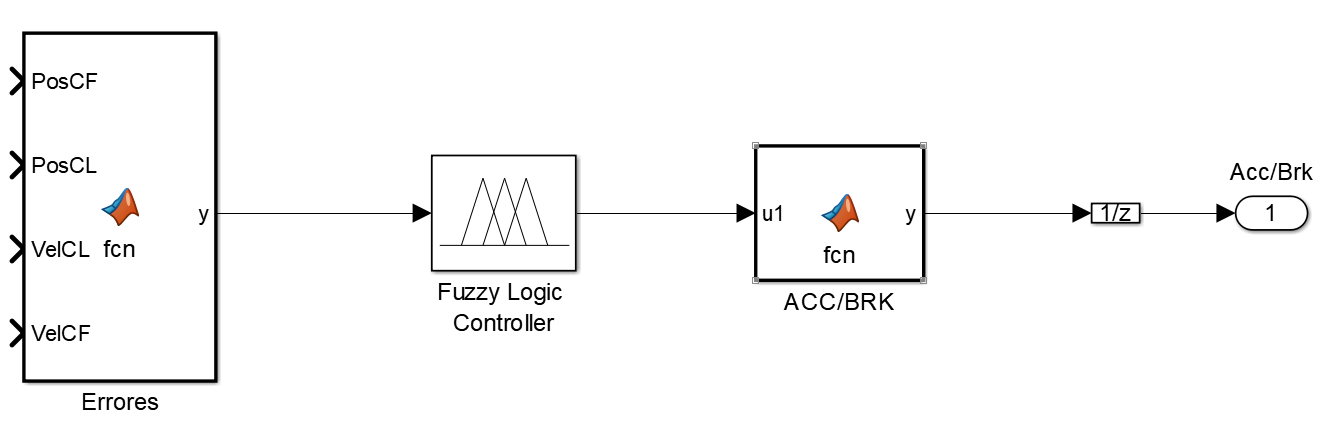
\includegraphics[scale=0.3]{Imagenes/accdyna}
		\caption{Implementación del ACC en Simulink}
		\label{fig:accdyna}
\end{figure}	 

\par Dentro del ToolBox se configuran las funciones de pertenencia, tanto de las entradas (Figuras \ref{fig:fuzzyvel} y \ref{fig:fuzzydist}), como de las salidas (Figura \ref{fig:fuzzyacc}), así como tambien las reglas planteadas. Cada elemento corresponde a un bloque del esquema que rige a los controladores difusos, siendo estos el de fuzzficación, defuzzyficación e inferencia, respectivamente, acotando que, como método de inferencia se empleó el de Mamdani y de defuzzyficación el del centroide, métodos establecidos como predeterminados en el ToolBox. 

\begin{itemize}

\item Función de Pertenencia del Error de Velocidad: para este parámetro se fijaron cuatro funciones, muy negativo, negativo, central y positivo, con el fin de ajustar de mejor forma la velocidad del vehículo, cuando este se encuentre cerca del valor de referencia. Además se adecuó el rango, de forma que no fuese muy amplio para tener un mejor control a velocidades bajas y medias. 

\begin{figure}[!h]
	\centering
		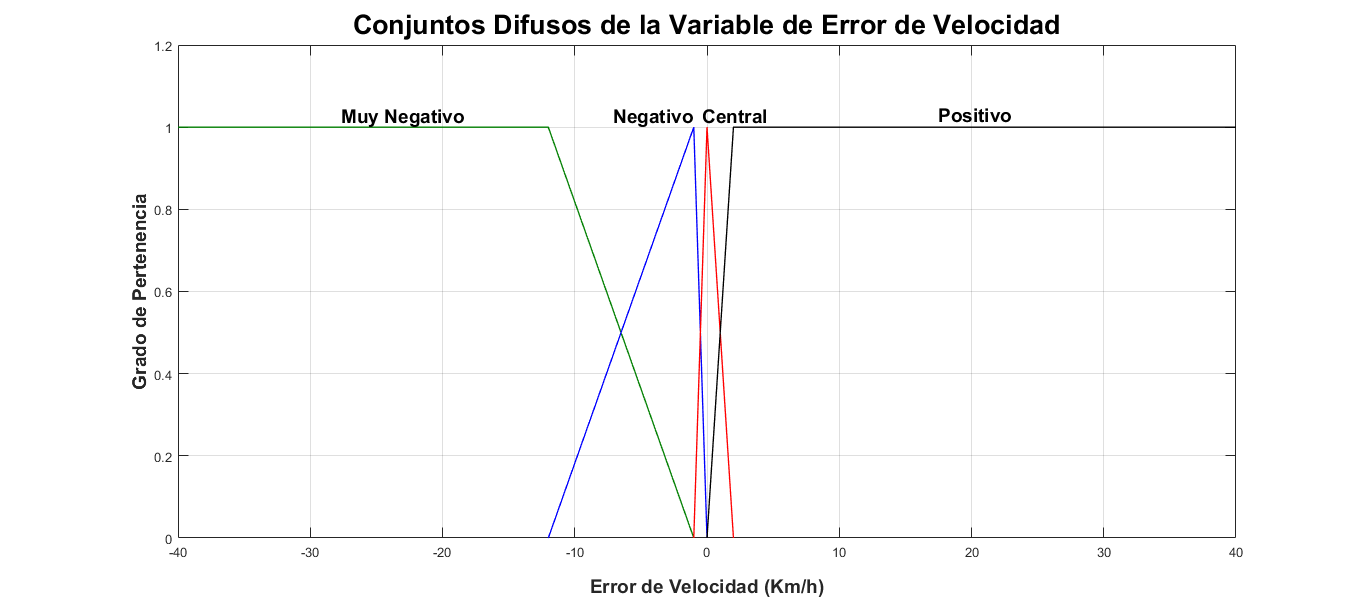
\includegraphics[scale=0.35]{Imagenes/fuzzyvel}
		\caption{Función de pertenencia del Error de Velocidad}
		\label{fig:fuzzyvel}
\end{figure}	 

\item Función de Pertenencia del Error de Distancia: para este parámetro de fijaron cuatro funciones, negativo, central, positivo y muy positivo, con el fin de ajustar la relación de distancia, de la misma forma que en el error de la velocidad para mantener el error cerca de la referencia, sin cambios bruscos.

\begin{figure}[!h]
	\centering
		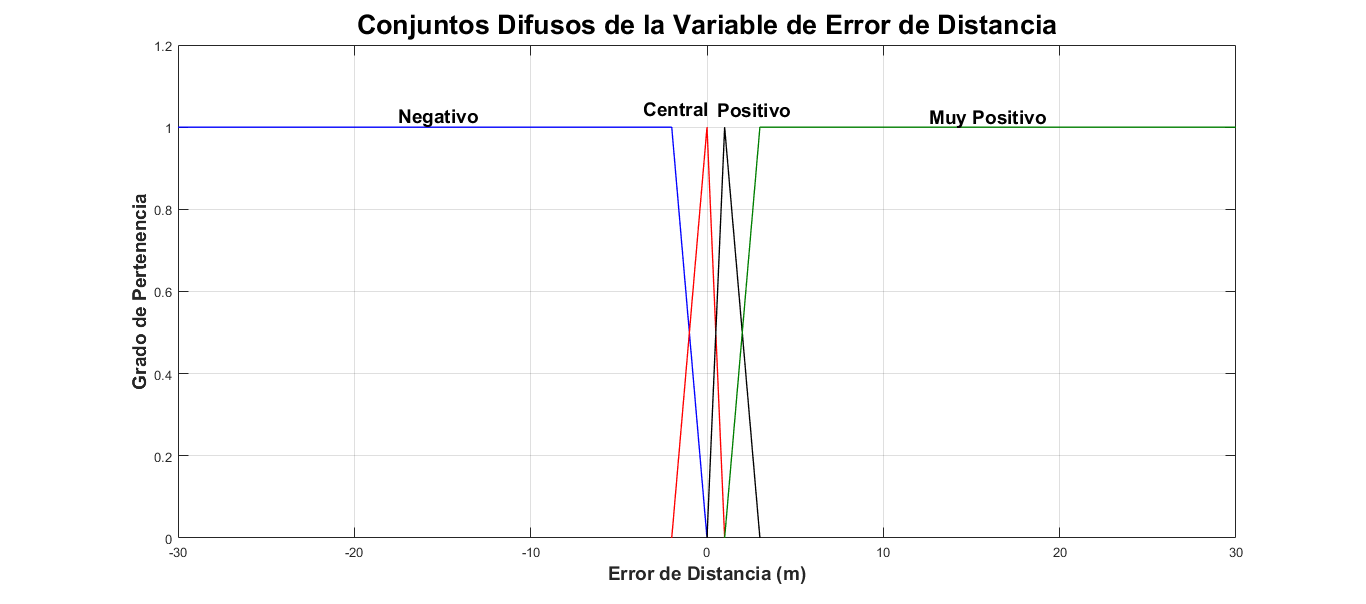
\includegraphics[scale=0.35]{Imagenes/fuzzydist}
		\caption{Función de pertenencia del Error de Distancia}
		\label{fig:fuzzydist}
\end{figure}	 

\end{itemize}
   
\par Dichos parámetros se seleccionaron utilizando la lógica experimental, observando los resultados obtenidos previamente y analizando la manera en que el controlador debería modificar la referencia de velocidad y distancia, según sea el escenario para lograr el objetivo planteado. Las reglas se constituyen de la siguiente forma:\\

	\hspace*{2pt}IF ErrorVel $Negativo$ AND ErrorDist $Positivo$ THEN ACC/BRK $NADA$\\
	\hspace*{20pt}IF ErrorVel $Negativo$ AND ErrorDist $Central$ THEN ACC/BRK $BRK$\\
	\hspace*{20pt}IF ErrorVel $Negativo$ AND ErrorDist $Negativo$ THEN ACC/BRK $BRKH$\\
	\hspace*{20pt}IF ErrorVel $Nada$ AND ErrorDist $Negativo$ THEN ACC/BRK $BRK$\\
	\hspace*{20pt}IF ErrorVel $Nada$ AND ErrorDist $Nada$ THEN ACC/BRK $NADA$\\
	\hspace*{20pt}IF ErrorVel $Nada$ AND ErrorDist $Positivo$ THEN ACC/BRK $ACC$\\
	\hspace*{20pt}IF ErrorVel $Positivo$ AND ErrorDist $Negativo$ THEN ACC/BRK $NADA$\\
	\hspace*{20pt}IF ErrorVel $Positivo$ AND ErrorDist $Nada$ THEN ACC/BRK $ACC$\\
	\hspace*{20pt}IF ErrorVel $Positivo$ AND ErrorDist $Positivo$ THEN ACC/BRK $ACCH$\\
	\hspace*{20pt}IF ErrorVel $MuyNegativo$ THEN ACC/BRK $BRKH$\\
	\hspace*{20pt}IF ErrorDist $MuyPositivo$ THEN ACC/BRK $ACCH$\\

\par En el caso de la salida, la misma esta contituida por 5 valores del tipo \textit{singleton} dentro del conjunto $\in$ [-1;1], donde los valores negativos corresponden al freno, y los positivos al acelerador. De la misma forma que para las entradas, los valores de salida se definieron de manera experimental, observando los resultados a medida que se modificaban los valores progresivamente.\\

\begin{figure}[!h]
	\centering
		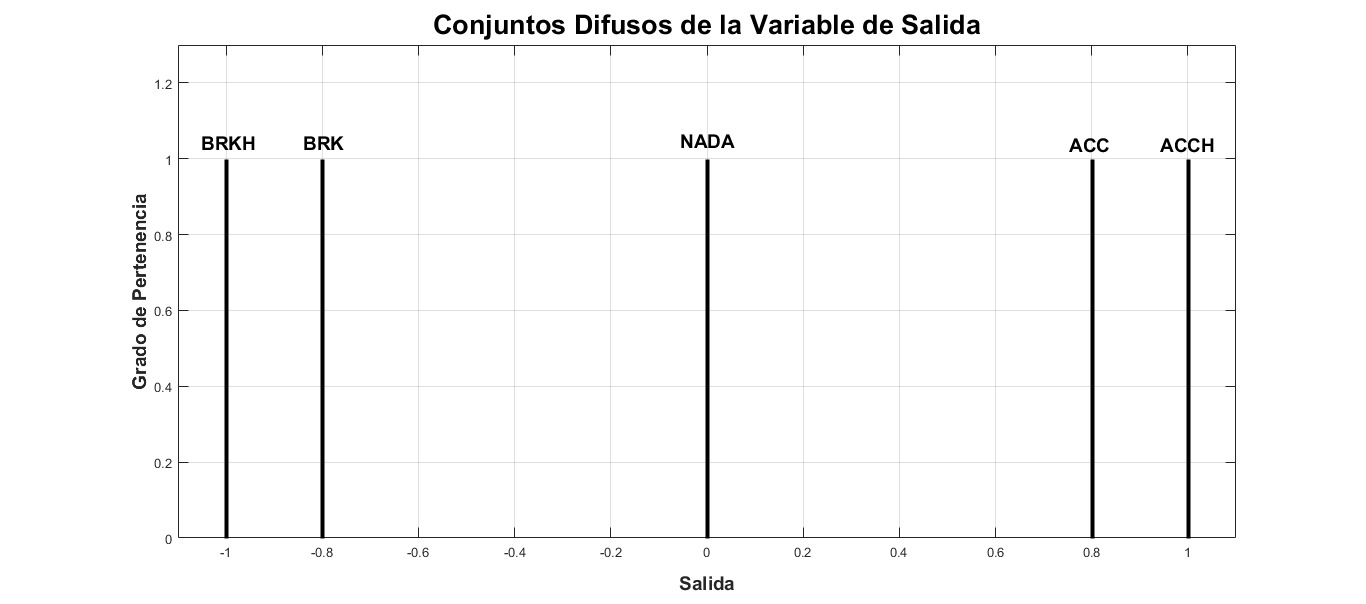
\includegraphics[scale=0.30]{Imagenes/fuzzyacc}
		\caption{Función de pertenencia de la Salida del Controlador}
		\label{fig:fuzzyacc}
\end{figure}	 

\par La configuración completa de las salidas, junto a las funciones de pertenencia y a las reglas dan como resultado la siguiente superficie de control (Figura \ref{fig:supacc}), mediante la cual se puede predecir el comportamiento exacto del controlador a partir de ambas entradas.\\

\begin{figure}[!h]
	\centering
		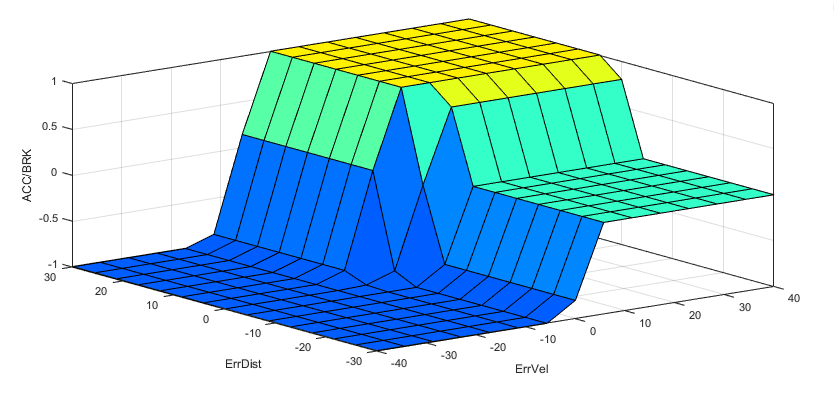
\includegraphics[scale=0.4]{Imagenes/supacc}
		\caption{Superficie de control generada}
		\label{fig:supacc}
\end{figure}	 

\subsection{Pruebas en Dynacar a Distintas Velocidades}

Para las pruebas de este controlador se emplearon dos módulos de Dynacar en un mismo diagrama de Simulink (Figura \ref{fig:dyna2}), con el cual se simulan dos vehículos en una misma computadora, ignorando los efectos que pueda introducir el módulo de comunicación, y de esta forma analizar con más certeza el desempeño del controlador. 

\begin{figure}[!h]
	\centering
		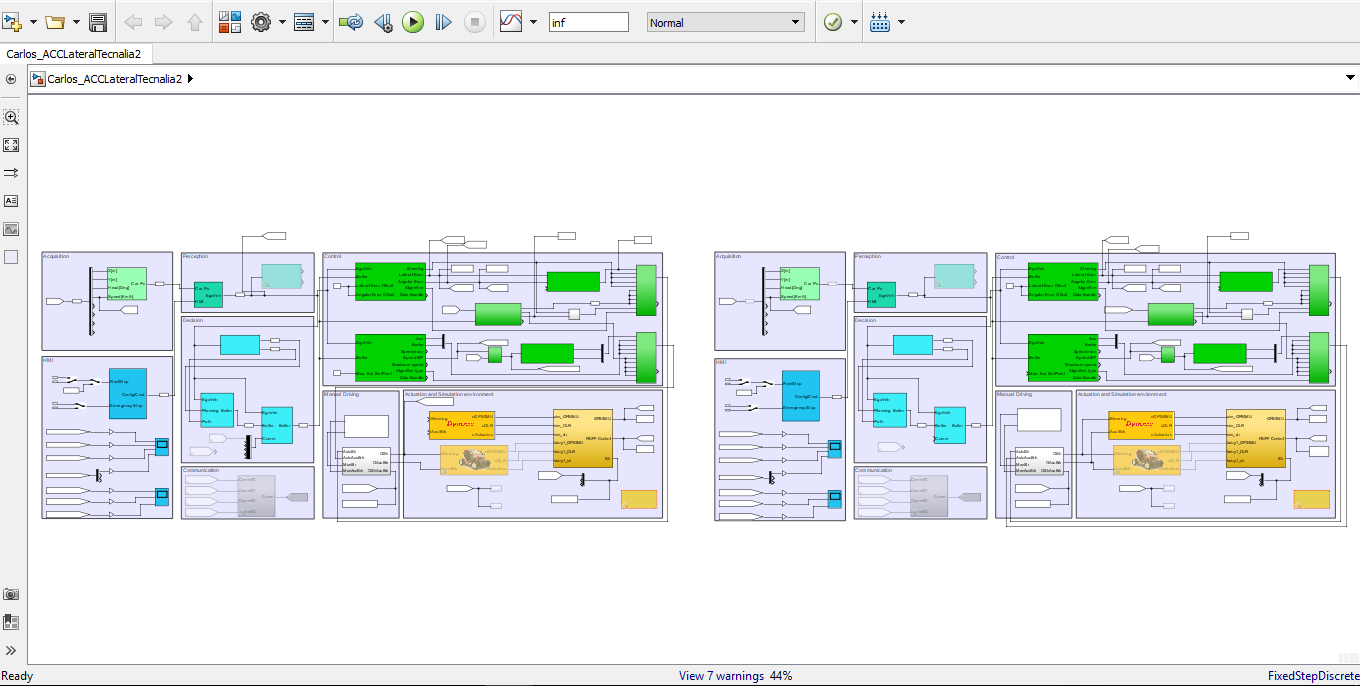
\includegraphics[scale=0.30]{Imagenes/dyna2}
		\caption{Diagrama de Simulink con dos módulos de Dynacar}
		\label{fig:dyna2}
\end{figure}	 

\par Así pues, se devidió las pruebas según la velocidad propuesta, siendo estas, velocidades bajas y velocidades medias.
%%%%%%%%%%%%%%%%%%%%%%%
\subsubsection{Velocidades Bajas}
%%%%%%%%%%%%%%%%%%%%%%%
En las Figuras \ref{fig:velvb} y \ref{fig:distvb} se puede encontrar el comportamiento del controlador a velocidades bajas, las cuales son establecidas en el rango de 10 Km/h a 30 Km/h. Más específicamente se observan las velocidades de los vehículos y la distancia entre los mismos.\\

\begin{figure}[H]
	\centering
		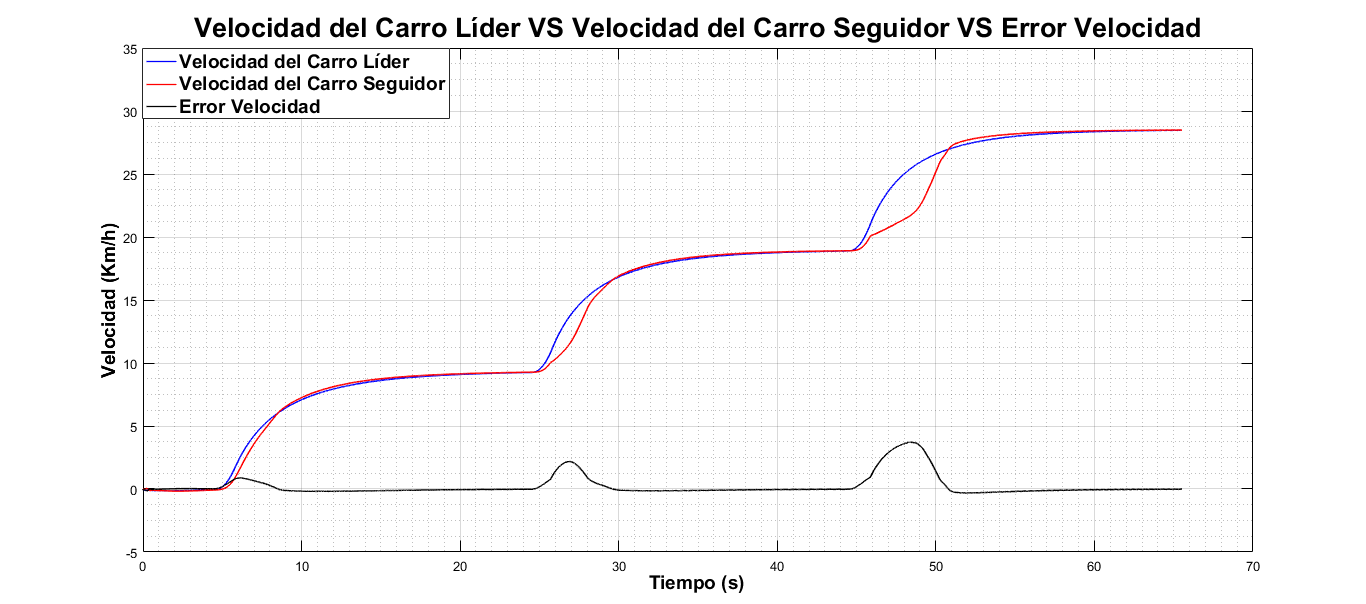
\includegraphics[scale=0.35]{Imagenes/accvb}
		\caption{Gráfica de la velocidad de los vehículos}
		\label{fig:velvb}
\end{figure}	

\begin{figure}[H]
	\centering
		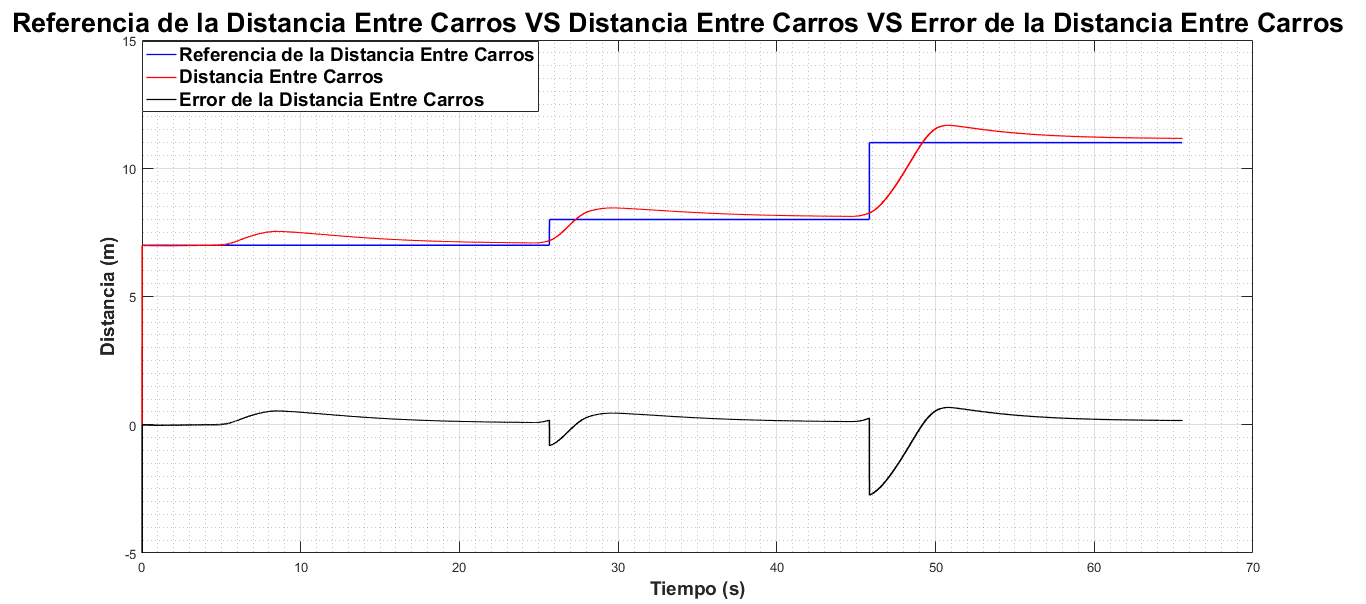
\includegraphics[scale=0.35]{Imagenes/accvmdist}
		\caption{Gráfica del error de la distancia de los vehículos}
		\label{fig:distvb}
\end{figure}	

\par Observando la Figura \ref{fig:velvb} se puede apreciar que tanto a 10 Km/h, como a 20 Km/h el vehículo seguidor se apega correctamente a la velocidad del líder, mostrando un error de 2 Km/h, al realizar el cambio de velocidad, mientras que en el cambio a 30 Km/h se presenta un error mayor, de 4 Km/h, el cual sigue siendo aceptable, logrando corregirse en un tiempo de 5 s. En lo que respecta a la distancia, la Figura \ref{fig:distvb}, muestra que el error máximo que se presenta es de 50 cm, con respecto a la referencia, y que tarda 10 s, en alcanzar dicho valor.

%%%%%%%%%%%%%%%%%%%%%%%
\subsubsection{Velocidades Medias}
%%%%%%%%%%%%%%%%%%%%%%%

En las Figuras \ref{fig:velvm} y \ref{fig:distvm} se puede encontrar el comportamiento del controlador a velocidades medias, las cuales son establecidas en el rango de 40 Km/h a 60 Km/h. De igual forma, se observan las velocidades de los vehículos y la distancia entre los mismos.

\begin{figure}[H]
	\centering
		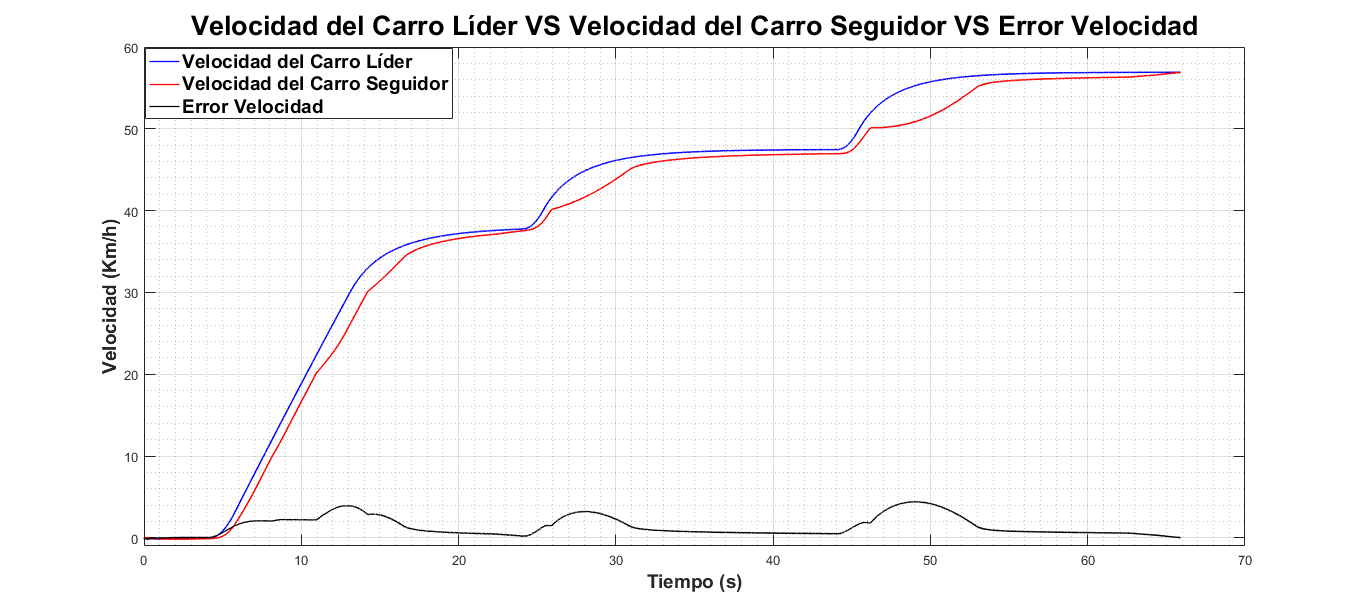
\includegraphics[scale=0.35]{Imagenes/accvm}
		\caption{Gráfica de la velocidad de los vehículos}
		\label{fig:velvm}
\end{figure}	

\begin{figure}[H]
	\centering
		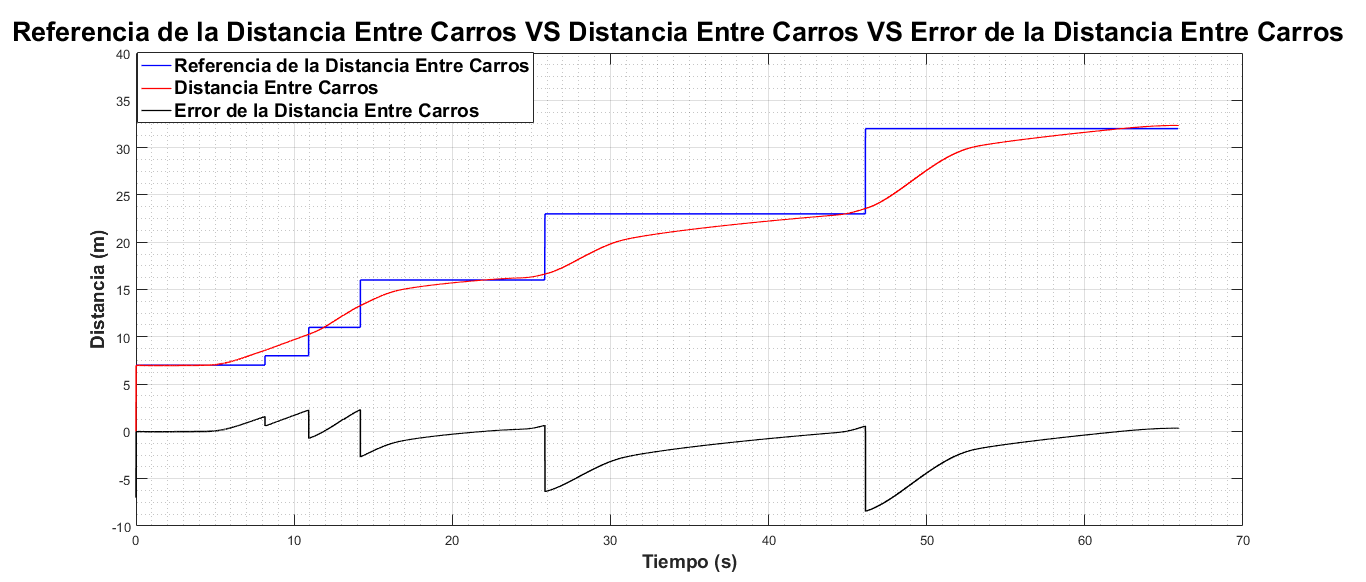
\includegraphics[scale=0.35]{Imagenes/accvbdist}
		\caption{Gráfica del error de la distancia de los vehículos}
		\label{fig:distvm}
\end{figure}	

\par En lo que respecta a la Figura \ref{fig:velvm} se puede apreciar que los errores al alcanzar la referencia aumentan, resultando en 0.5 Km/h por debajo de la velocidad del vehículo líder, siendo esto un error equivalente al 1 \%, mientras que para alcanzar el valor de rerencia se manetiene el error de 2 Km/h. El tiempo de establecimiento es de 14 s, 4 segundos más que el que tarda para estabilizarce en las velocidades bajas 


%%%%%%%%%%%%%%%%%%%%%%%%%%%%%%%%%%%%%%%%%
\section{Control Lateral}
%%%%%%%%%%%%%%%%%%%%%%%%%%%%%%%%%%%%%%%%%
Esta maniobra busca mantener la posición y dirección, tomando en cuenta la posición del carro que tiene al frente. Para conseguir esto, se realizó un controlador difuso\cite{sriranjanlateral} que recibe como entradas el error lateral y el error angular, y como salida, el ángulo que debe mantener el volante.  

\subsection{Algoritmo de Control}

Para el cálculo de los errores se emplea la posición del vehículo líder, con la cual se arma un vector de 150 valores, que se actualiza cada 50 ms, donde además, se guarda la dirección del vehículo en dichos puntos. Con estos valores se compara la posición y dirección del vehículo seguidor, pudiendo así obtener el error lateral y angular (Figura \ref{fig:cle}). 


\begin{figure}[!h]
	\centering
		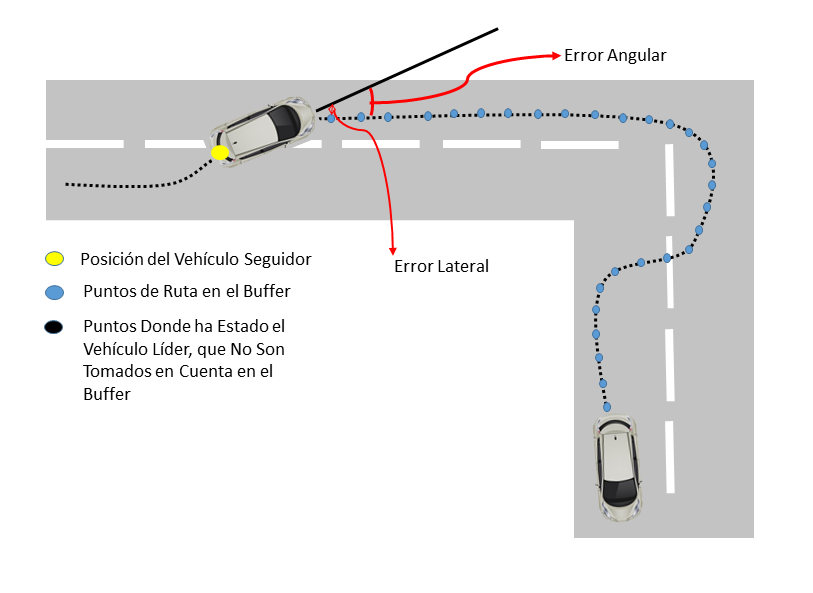
\includegraphics[scale=0.40]{Imagenes/cle}
		\caption{Caractrísticas del Control Lateral implementado}
		\label{fig:cle}
	\end{figure}	 

Entonces, proyectando la posición del vehículo la posción a las ruedas delanteras, se tiene que los errores son calculados de la siguiente forma:

\begin{itemize}

\item Error Lateral: para el cálculo del error lateral se toma en cuenta, que el mismo es la distancia que existe entre el punto de control delantero hasta el segemento de recta en el cual se encuentra el vehículo. Con esto dicho, se busca un punto de esta recta que se ecnuentre más cerca a la pocisión del vehículo y se calcula el error, con la siguiente fórmula: 

\par Proyección de la posición del vahículo al punto de control delantero (\textit{Lookahead}):

\begin{equation} \label{eq:distel}
X = Lookahead\cdot \cos({\textit{heading}})
\end{equation}
\begin{equation} \label{eq:distel}
Y = Lookahead\cdot \sen({\textit{heading}})
\end{equation}
\par Error lateral:
\begin{equation} \label{eq:distel}
E_{Lat} = \sqrt{(X_{VS}-X_{Seg})^{2} + (Y_{VS}-Y_{Seg})^{2}}
\end{equation}

\par Para saber la orientación del error, se calcula el producto escalar, de los vectores formados por la posición del vehículo y el segmento de recta, valor, que sí resulta positivo, quiere decir que el vehículo se encuentra a la derecha de la recta, mientras que si es negativo, se encuentra a la izquierda.

\item Error Angular: para el cálculo de este error, se toma en consideración, que el mismo es las desviación del ángulo del vehículo, con respecto al segmento, el cual puede tomar valores entre [-$\pi$;$\pi$], así pues, el error se calcula el error de la siguiente forma:

\begin{equation} \label{eq:distang}
E_{Ang} = \arctan{\frac{\sen{\psi_{VS}}}{\cos{\psi_{VS}}}} - \arctan{\frac{\sen{\psi_{VL}}}{\cos{\psi_{VL}}}}
\end{equation}
 
\par Valor que si resulta positivo indica que la dirección del vehículo está a la derecha con respecto a la del segmento, mientras que si es negativo se encuentra direccionado a la izquierda. 
\end{itemize}

\subsection{Implementación en el Simulador}

Para la implementación en Dynacar también se hizo uso del ToolBox de Matlab para controladores difusos, al cual se le pasa como entradas el error lateral y el error angular, y tiene como salida el ángulo del volante (Figura \ref{fig:cldyna})


\begin{figure}[!h]
	\centering
		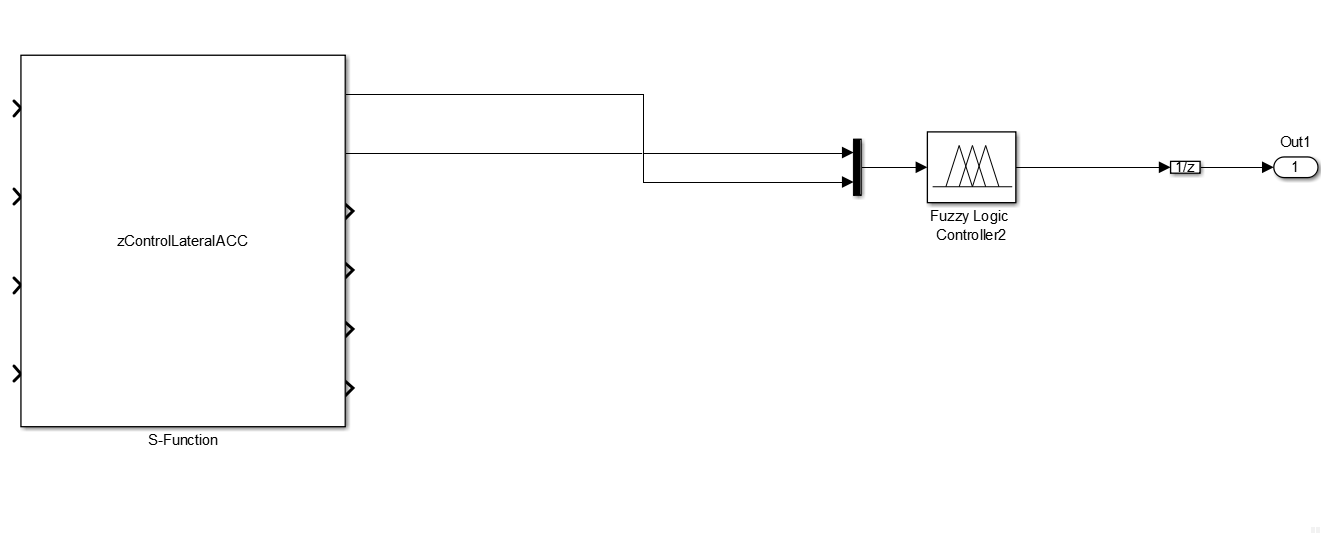
\includegraphics[scale=0.3]{Imagenes/cldyna}
		\caption{Implementación del Control Lateral en Simulink}
		\label{fig:cldyna}
\end{figure}	 

\par De la misma forma se configuraron las funciones de pertenencia de entrada (Figuras \ref{fig:fuzzylat} y \ref{fig:fuzzyang}) y de salida (Figura \ref{fig:clsal}), así como las reglas planteadas, además de emplear el método de inferencia y de desfuzzyficación que el controlador del ACC.

\begin{itemize} 

\item Función de pertenencia del Error Lateral: para este parámetro se fijaron tres funciones, negativo, central y positivo, con una apertura central grande para no mantener el vehículo lo más centrado posible, sin generar cambios bruscos.

\begin{figure}[!h]
	\centering
		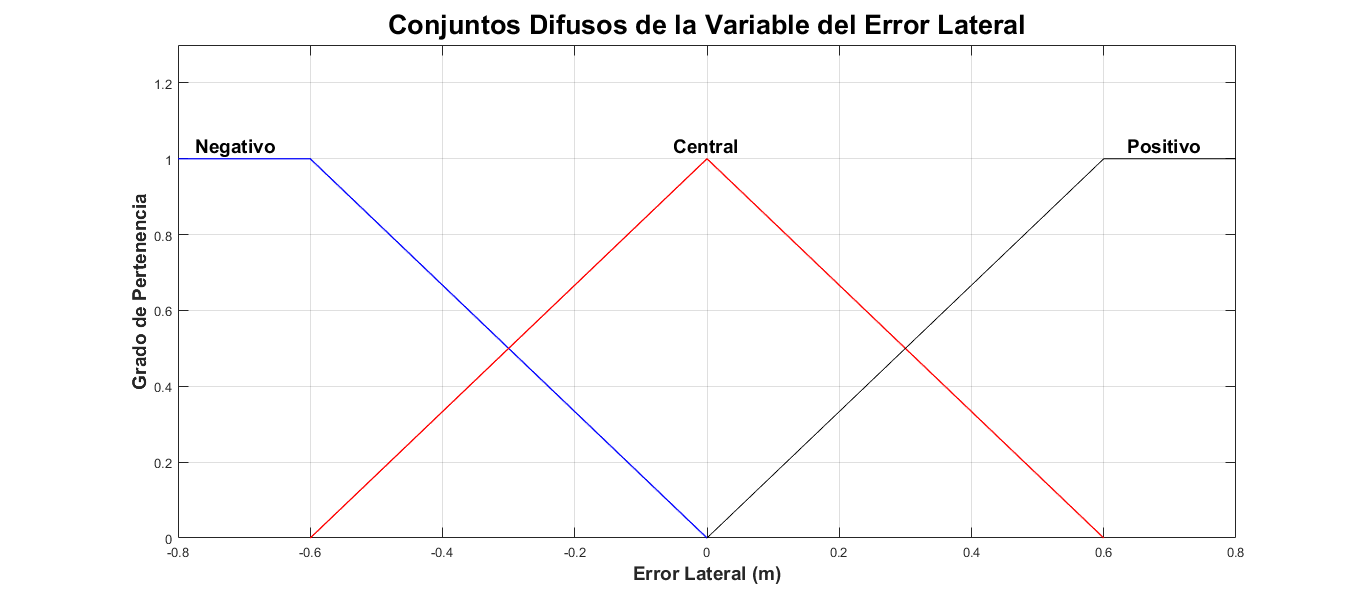
\includegraphics[scale=0.29]{Imagenes/fuzzylat}
		\caption{Función de pertenencia del Error Lateral}
		\label{fig:fuzzylat}
\end{figure}	 



\item Función de pertenencia del Error Angular: para este parámetro se fijaron tres funciones, negativo, central y positivo, con una apertura central grande para no mantener la dirección del vehículo lo más cercana posible a la del vehículo líder, sin generar cambios abruptos.

\begin{figure}[!h]
	\centering
		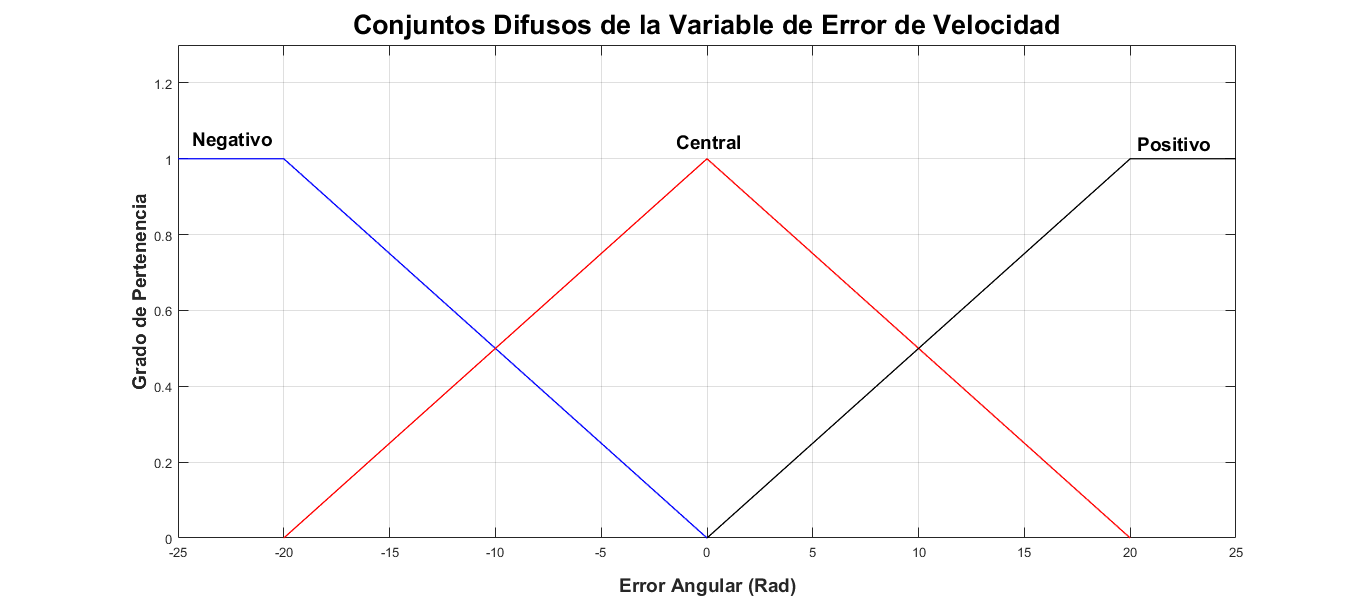
\includegraphics[scale=0.29]{Imagenes/fuzzyang}
		\caption{Función de pertenencia del Error Angular}
		\label{fig:fuzzyang}
\end{figure}	 
\end{itemize}

\par Al igual que con el controlador del ACC, estos parámetros fueron seleccionados utiliando la lógica experimental, observando su comportamiento y ajustándolo según sea necesario. Las reglas planteadas son las siguientes:\\

	\hspace*{2pt}IF ErrorAng $Negativo$ AND ErrorDist $Negativo$ THEN Steering $HIzquierda$\\
	\hspace*{20pt}IF ErrorAng $Negativo$ AND ErrorDist $Central$ THEN Steering $MIzquierda$\\
	\hspace*{20pt}IF ErrorAng $Negativo$ AND ErrorDist $Positivo$ THEN Steering $Izquierda$\\
	\hspace*{20pt}IF ErrorAng $Central$ AND ErrorDist $Negativo$ THEN Steering $LIzquierda$\\
	\hspace*{20pt}IF ErrorAng $Central$ AND ErrorDist $Central$ THEN Steering $Central$\\
	\hspace*{20pt}IF ErrorAng $Central$ AND ErrorDist $Positivo$ THEN Steering $LDerecha$\\
	\hspace*{20pt}IF ErrorAng $Positivo$ AND ErrorDist $Negativo$ THEN Steering $Derecha$\\
	\hspace*{20pt}IF ErrorAng $Positivo$ AND ErrorDist $Central$ THEN Steering $MDerecha$\\
	\hspace*{20pt}IF ErrorAng $Positivo$ AND ErrorDist $Positivo$ THEN Steering $HDerecha$\\

\par En el caso de la salida, la misma consta de 9 valores dentro del conjunto $\in$ [-0.6;0.6], donde los valores negativos corresponden a realizar giros del volante a la izquierda, y los positivos, giros a la derecha. Estos valores fueron fijados de manera experimental.\\ 

\begin{figure}[!h]
	\centering
		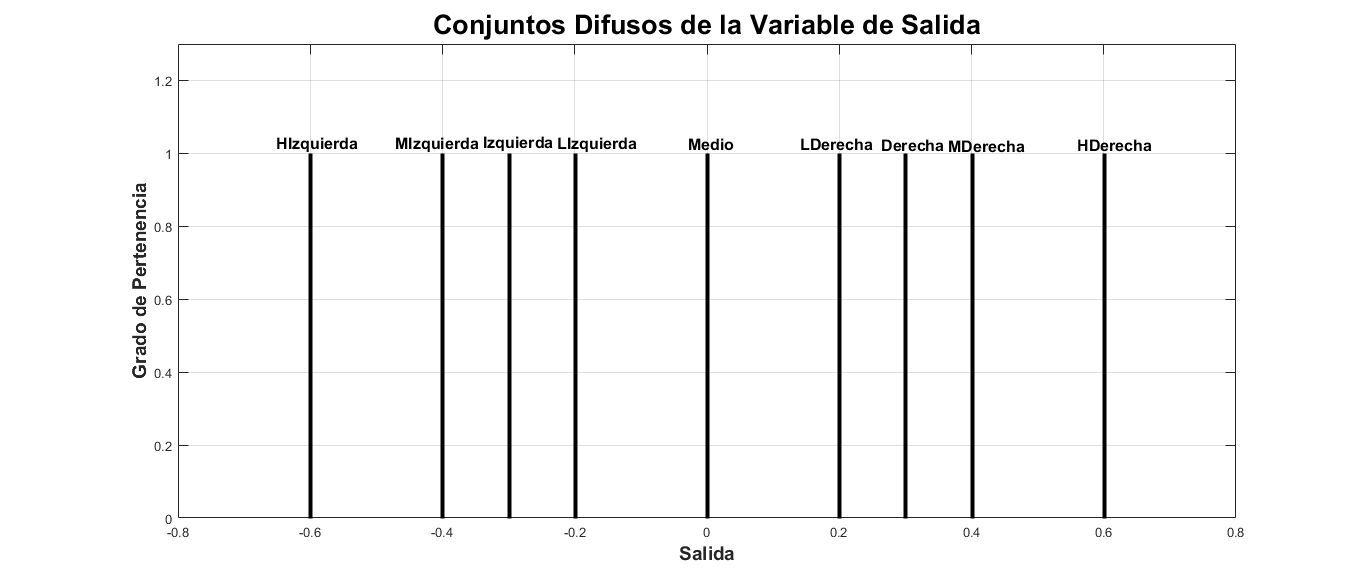
\includegraphics[scale=0.32]{Imagenes/clsal}
		\caption{Función de pertenencia de la Salida del Controlador}
		\label{fig:clsal}
\end{figure}	 

\par La configuración completa de las salidas, junto a las funciones de pertenencia y a las reglas dan como resultado la siguiente superficie de control (Figura \ref{fig:supacc}), mediante la cual se puede predecir el comportamiento del controlador a partir de ambas entradas.\\

\begin{figure}[!h]
	\centering
		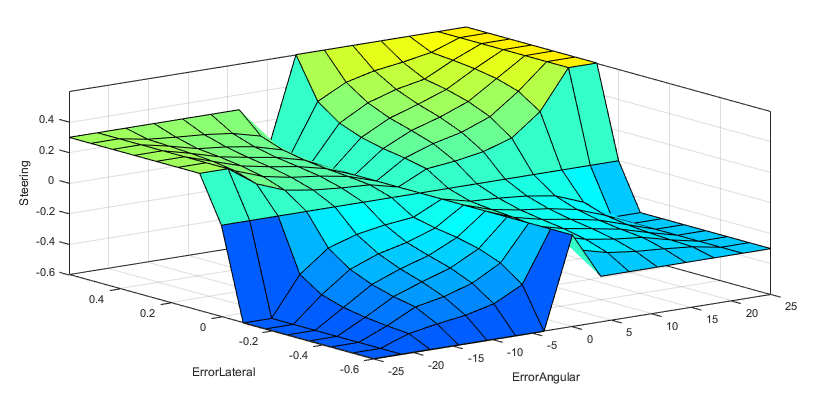
\includegraphics[scale=0.4]{Imagenes/supcl}
		\caption{Superficie de control generada}
		\label{fig:supcl}
\end{figure}	 


\subsection{Pruebas en Dynacar con Distintos Tipos de Curvas a Velocidad Constante}

Para las pruebas del controlador se emplearon dos módulos de Dynacar, obviando así los efectos de los módulos de comunicación. En este caso se utilizó como escenario, la pista presentada en TECNALIA \textit{Research \& Innovation} (Figura \ref{fig:tecnaliap2}). En dicha pista se peuden destacar tres tramos, el tramo uno, primera curva fuerte, tramo dos, cambio de carril, tramo tres una segunda curva más suave. Así pues, a continuación se muestra el desempeño del controlador, ante estos tramos:

\begin{figure}[!h]
	\centering
		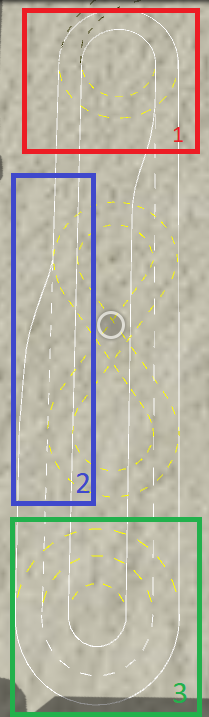
\includegraphics[scale=0.35]{Imagenes/tecnaliap2}
		\caption{Pista de TECNALIA \textit{Research \& Innovation}}
		\label{fig:tecnaliap2}
\end{figure}	 

%%%%%%%%%%%%%%%%%%%%%%%
\subsubsection{Cambio de Carril}
%%%%%%%%%%%%%%%%%%%%%%%
Es la prueba correspondiente al segundo segmento, en el cual se evalua el comportamiento del controlador ante un cambio de carril, en dicha prueba se realiza la comparación entre la ruta realizada por el vehículo líder, la ruta del vehículo seguidor, y la ruta establecida por el planificador local. 
%%%%%%%%%%

 \begin{figure}[H]
 \centering
  \subfloat[Gráfica de la ruta seguida por los vehículos]{
   \label{fig:vcc}
    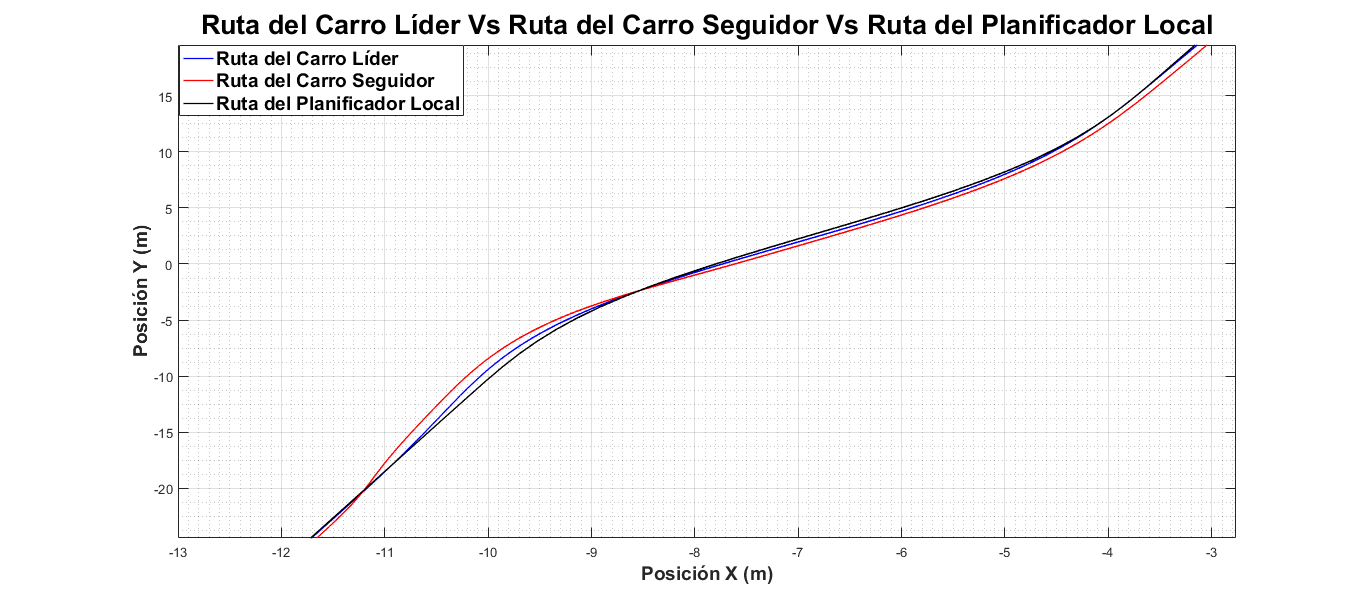
\includegraphics[scale=0.28]{Imagenes/rcc}}
  \subfloat[Ruta seguida por los vehículos en Dynacar]{
   \label{fig:dcc}
    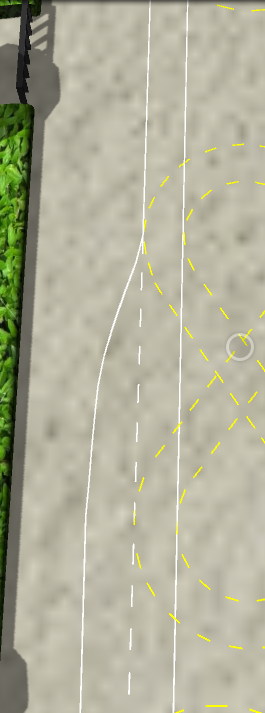
\includegraphics[scale=0.28]{Imagenes/dcf}}
 \caption{Ruta establecida para el cambio de carril}
 \label{fig:rcc}
\end{figure}

\par De la Figura \ref{fig:rcc} se puede apreciar que la ruta seguida por ambos vehículos es muy parecida a la ruta generada por el planificador local, encontrando una leve diferencia al efectuar el cambio de carril, aún así es una diferencia pequeña, como puede ser observada en las Figura Figuras \ref{fig:ccea} y \ref{fig:ccel}. Donde se muetra la comparación de las variables de control de ambos vehículos, teniendo, que el error lateral en ambos casos es de 15 cm, mientras que el error angular del vehículo seguidor es de 5.5 grados, 1.5 grados mayor que el del vehículo líder, produciendo que se tenga que jerecer una mayor acción sobre el volante.\\ 


\begin{figure}[H]
	\centering
		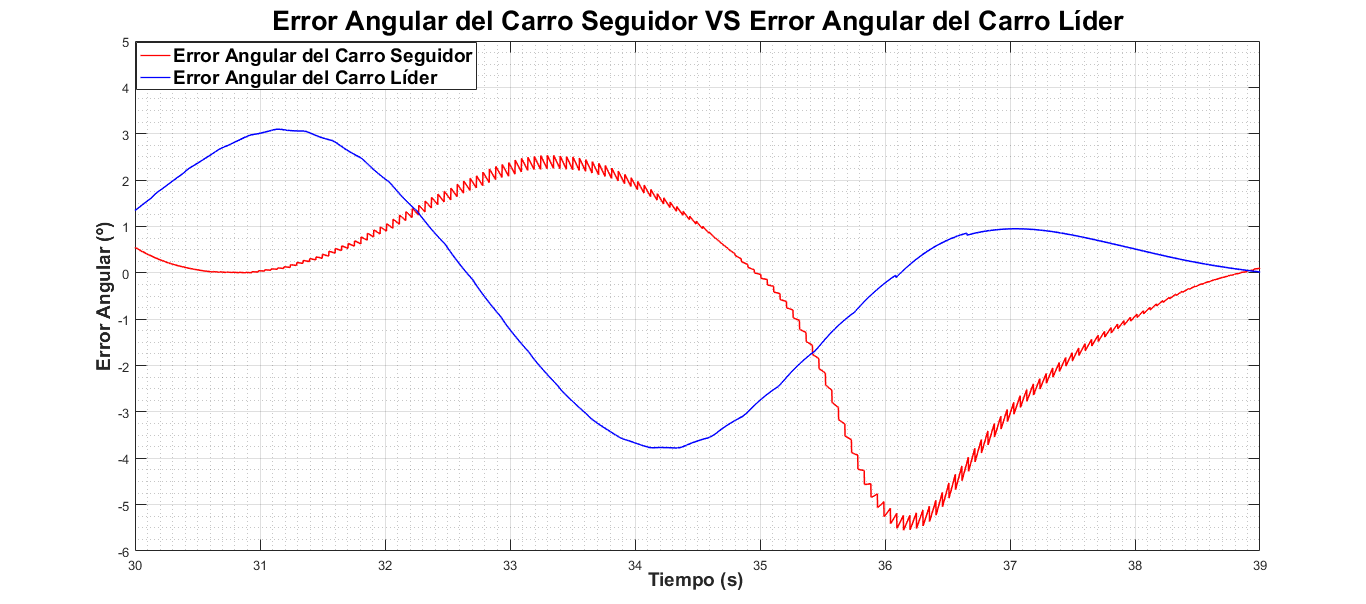
\includegraphics[scale=0.35]{Imagenes/ccea}
		\caption{Gráfica del error angular de los vehículos}
		\label{fig:ccea}
\end{figure}	

\begin{figure}[H]
	\centering
		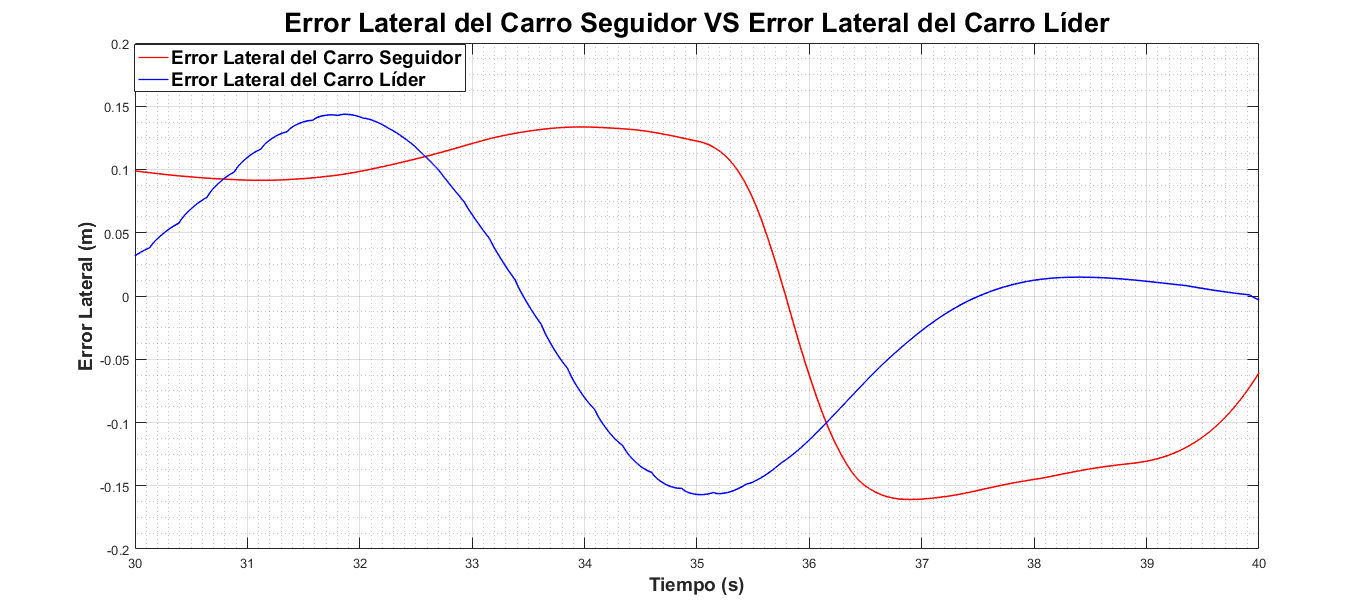
\includegraphics[scale=0.35]{Imagenes/ccel}
		\caption{Gráfica del error lateral de los vehículos}
		\label{fig:ccel}
\end{figure}	

%\begin{figure}[H]
%	\centering
%		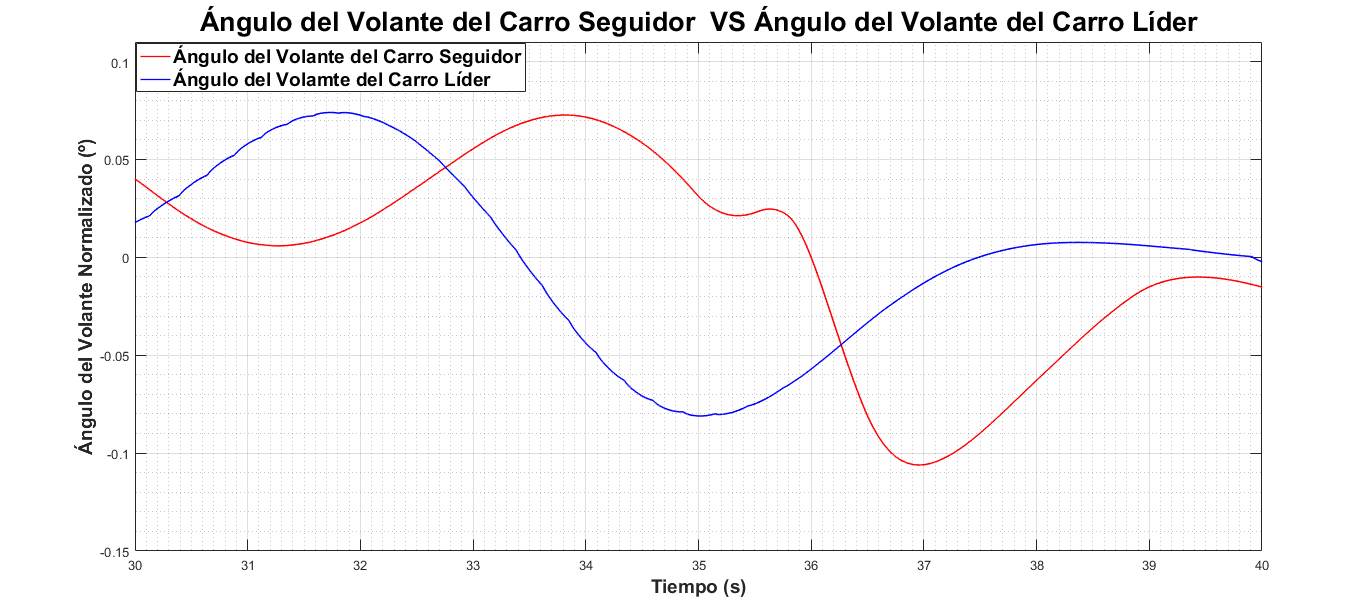
\includegraphics[scale=0.35]{Imagenes/ccst}
%		\caption{Gráfica del ángulo del volane de los vehículos}
%		\label{fig:ccst}
%\end{figure}	


%%%%%%%%%%%%%%%%%%%%%%%
\subsubsection{Curvas}
%%%%%%%%%%%%%%%%%%%%%%%
En este caso se presenta el segemento de curva uno, mostrando de igual forma la comparación de ruta seguida por ambos vehículos, así como la ruta esatblecida por el planificador local (Figura \ref{fig:rcf}). De dicha comparación se puede observar que la diferencia con la ruta del planificador local es alta, sin embargo no excede los límites del canal por el cual se circula. A pesar de esto, la diferencia de la ruta del carro seguidor con respecto al líder es baja.\\

 \begin{figure}[H]
 \centering
  \subfloat[Gráfica de la ruta seguida por los vehículos]{
   \label{fig:arvcf}
    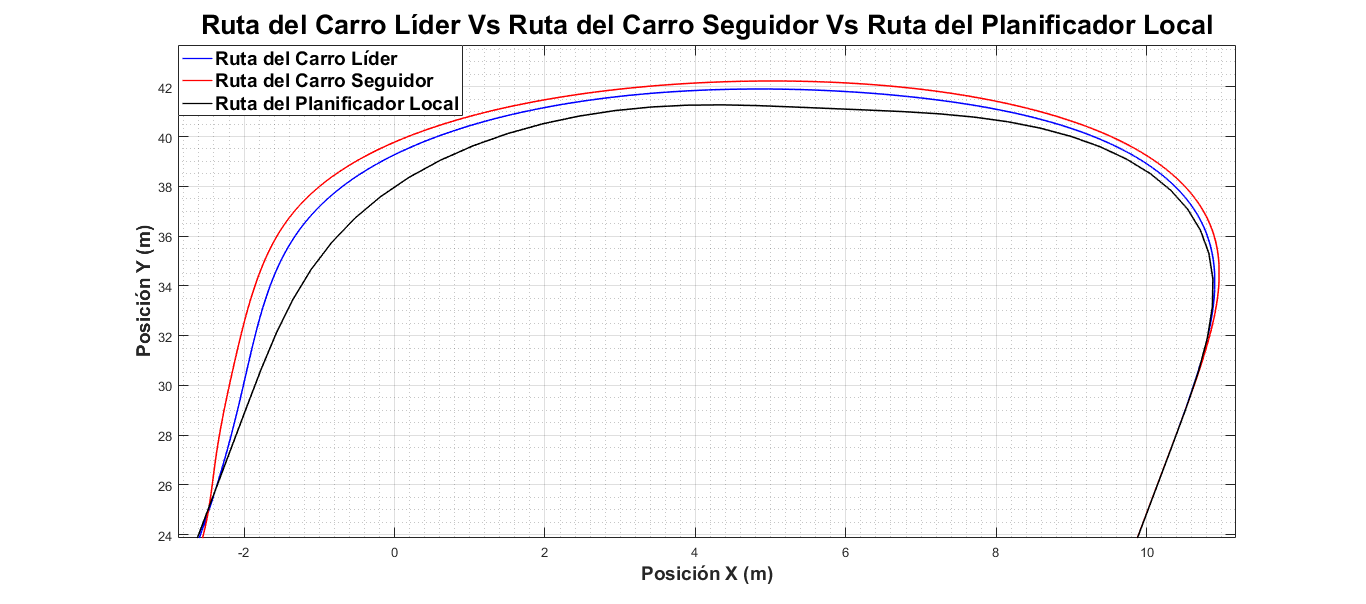
\includegraphics[scale=0.28]{Imagenes/rcf}}
  \subfloat[Ruta seguida por los vehículos en Dynacar]{
   \label{fig:vrdcf}
    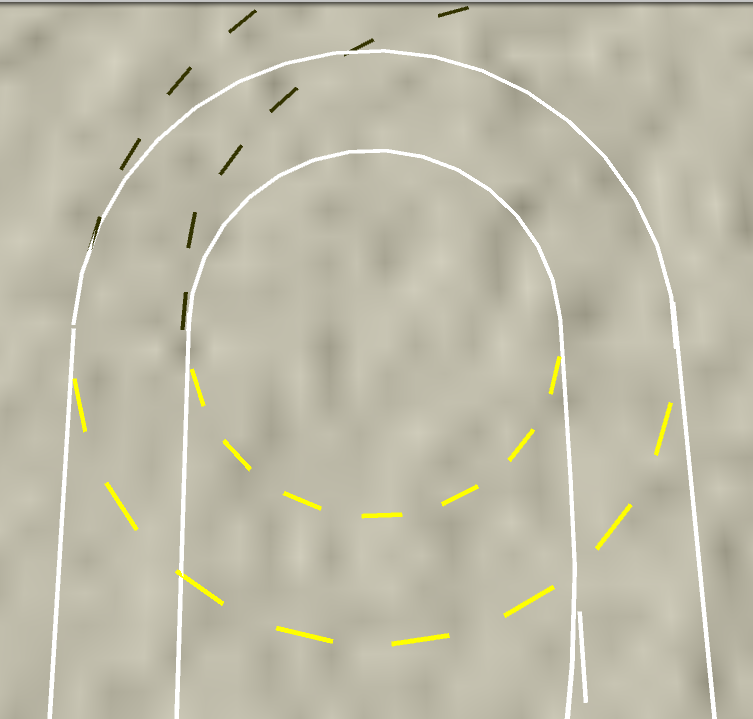
\includegraphics[scale=0.28]{Imagenes/dcc}}
 \caption{Ruta establecida para las curvas fuertes}
 \label{fig:rcf}
\end{figure}

\par En cuanto a los errores (Figuras \ref{fig:cfea} y \ref{fig:cfel}), se puede apreciar que tanto el error lateral como el angular (58 cm, y 20 grados repectivamente) del vehículo seguidor poseen un valor menor al del líder (1.01 m y 28 grados), lo cual indica que, según la ruta del vehículo líder el carro seguidor presenta un error bajo, pudiéndose corroborar con la Figura \ref{fig:rcf}, donde ambas rutas se asemejan en buena medida, viéndose separadas a la ruta del planificador local.\\

\begin{figure}[H]
	\centering
		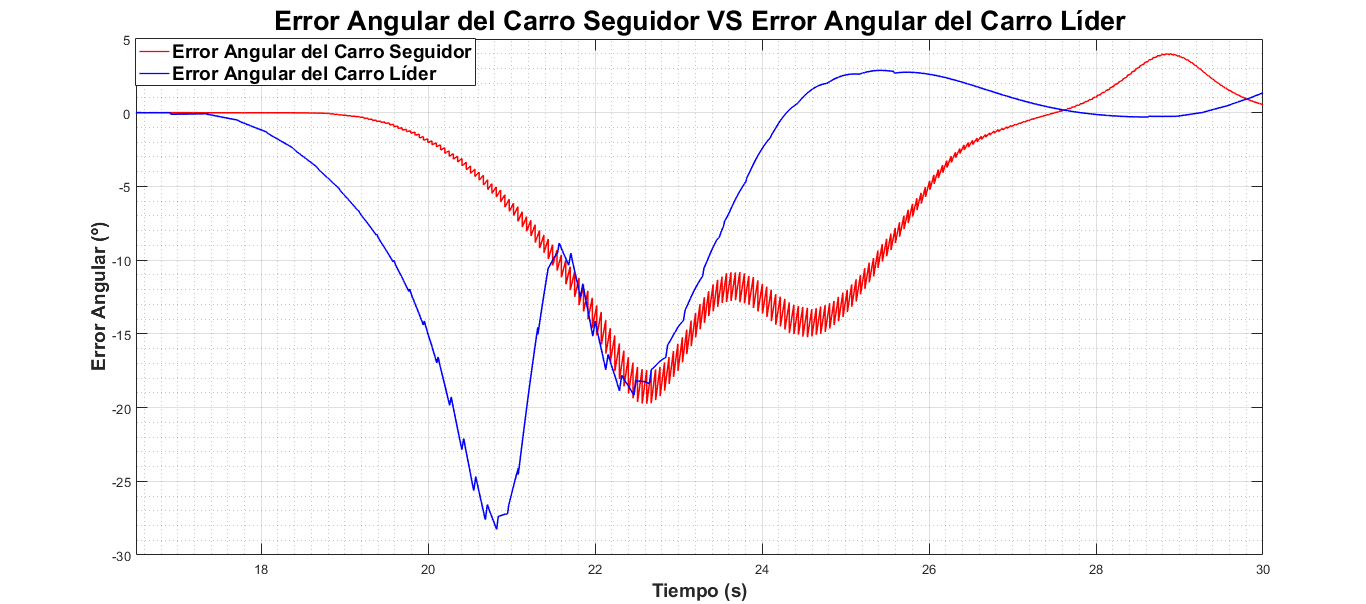
\includegraphics[scale=0.35]{Imagenes/cfea}
		\caption{Gráfica del error angular de los vehículos}
		\label{fig:cfea}
\end{figure}	

\begin{figure}[H]
	\centering
		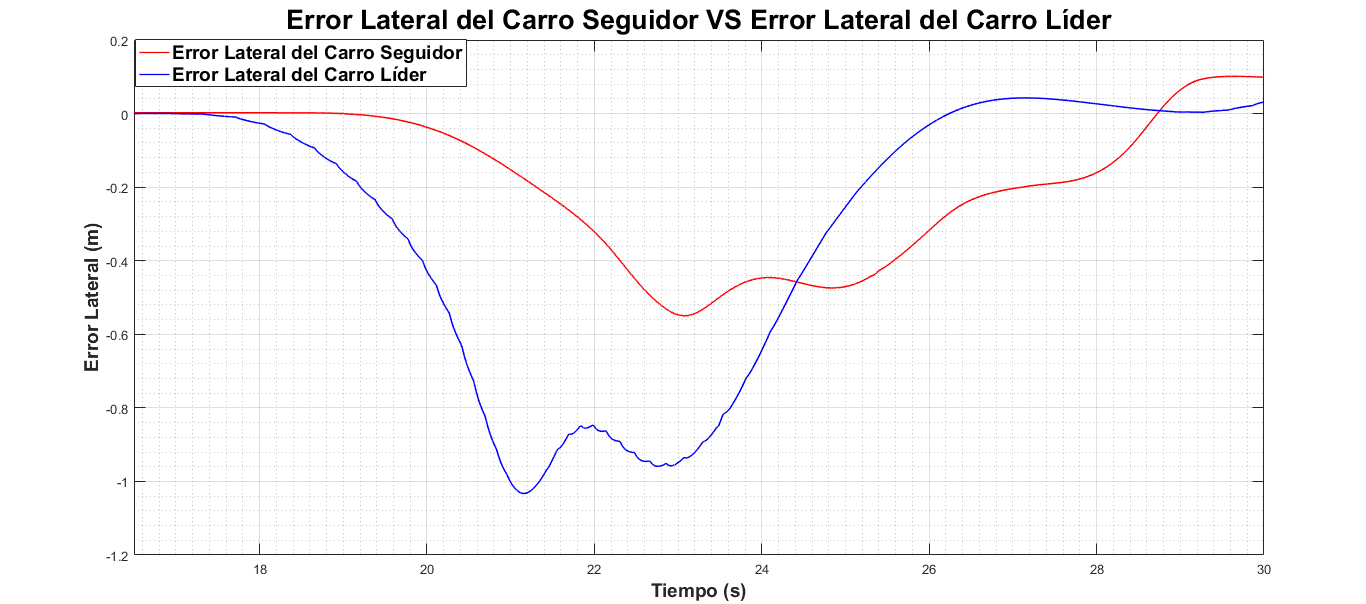
\includegraphics[scale=0.35]{Imagenes/cfel}
		\caption{Gráfica del error lateral de los vehículos}
		\label{fig:cfel}
\end{figure}	

%\begin{figure}[H]
%	\centering
%		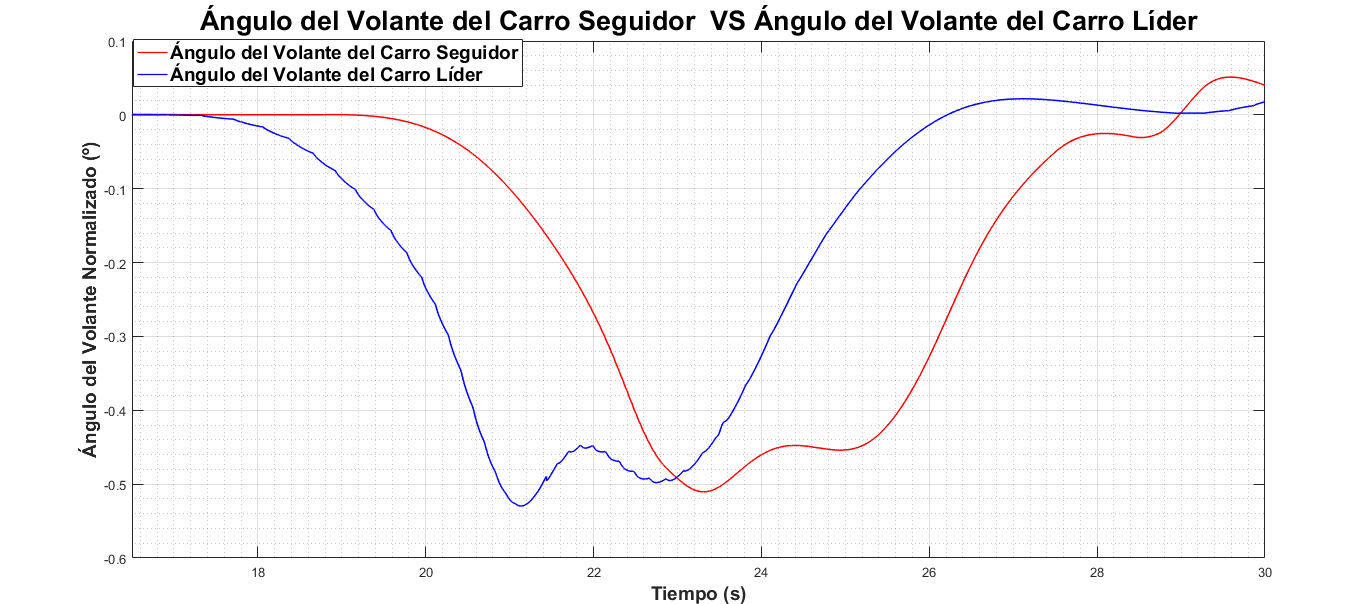
\includegraphics[scale=0.35]{Imagenes/cfst}
%		\caption{Gráfica del ángulo del volane de los vehículos}
%		\label{fig:cfst}
%\end{figure}	


\par En lo que respecta a la segunda curva (Figura \ref{fig:rcs}), se puede apreciar que las rutas seguida por ambos vehículos poseen mucha similitud, teniendo la mayor separación con respecto a la establecida por el planificador local en el tramo final de la curva, que se puede deber a la configuración del controlador del carro líder. \\  

\begin{figure}[H]
 \centering
  \subfloat[Gráfica del la ruta seguida por los vehículos]{
   \label{fig:vcs}
    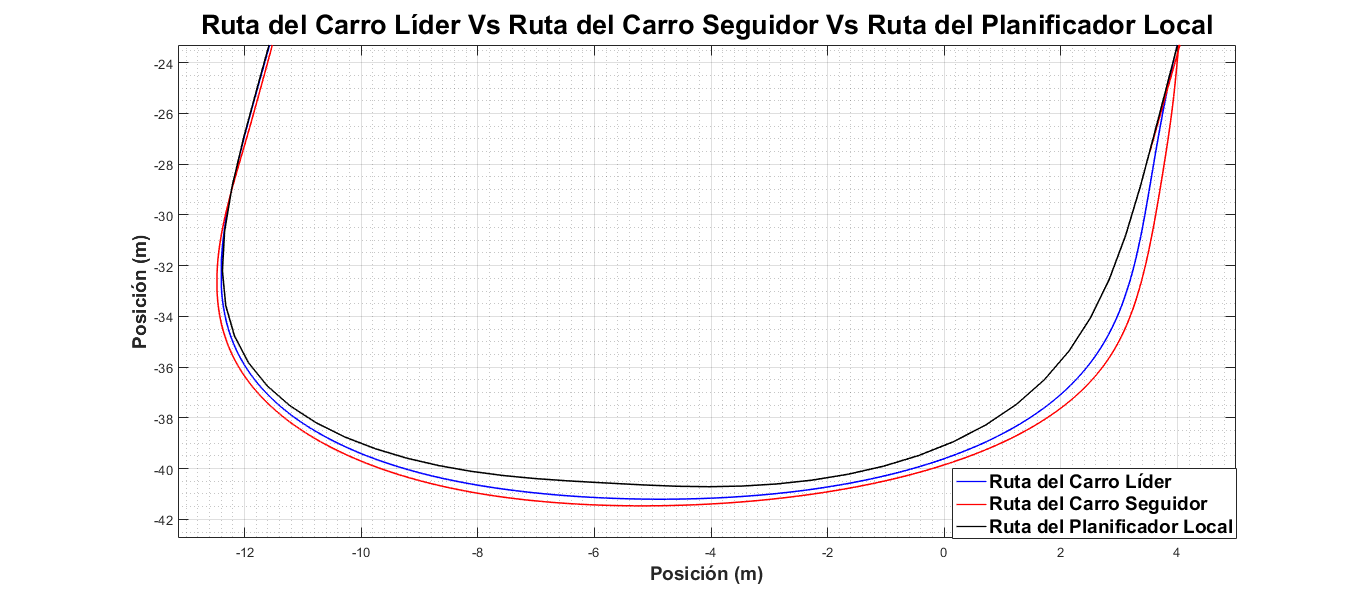
\includegraphics[scale=0.28]{Imagenes/rcs}}
  \subfloat[Ruta seguida por los vehículos en Dynacar]{
   \label{fig:dcs}
    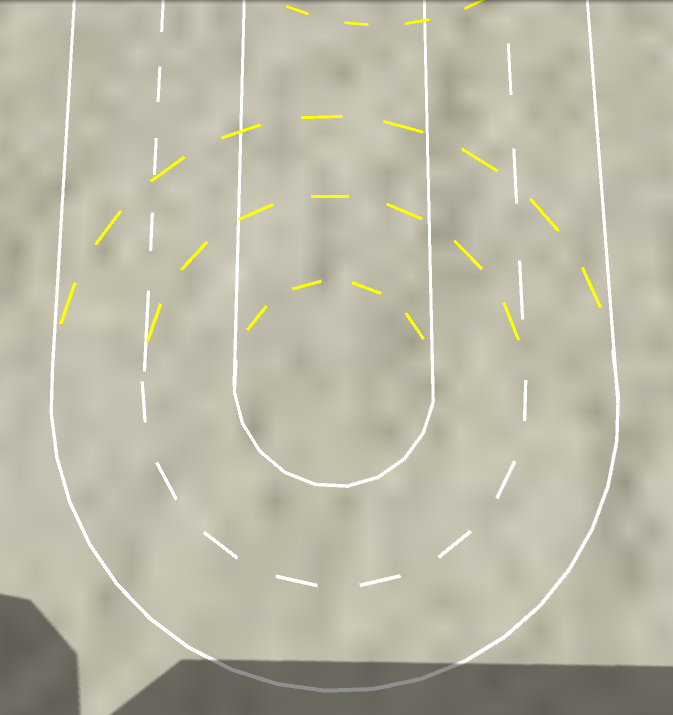
\includegraphics[scale=0.28]{Imagenes/dcs}}
 \caption{Ruta establecida para las curvas suaves}
 \label{fig:rcs}
\end{figure}

\par A pesar de esta diferencia en las rutas, ambos vehículos se encuentran dentro del carril, lo que implica que poseen un buen comportamiento. Afirmación que se puede confirmar con las Figuras \ref{fig:csea} y \ref{fig:csel}, en donde los errores laterales de los vehículos son menores a 1 metro, y más aún los errores, tanto angular como lateral del vehículo seguidor son menores a los presentados por el líder, logrando de esta forma un recorrido bastante similar, como fue comentado anteriormente.

\begin{figure}[H]
	\centering
		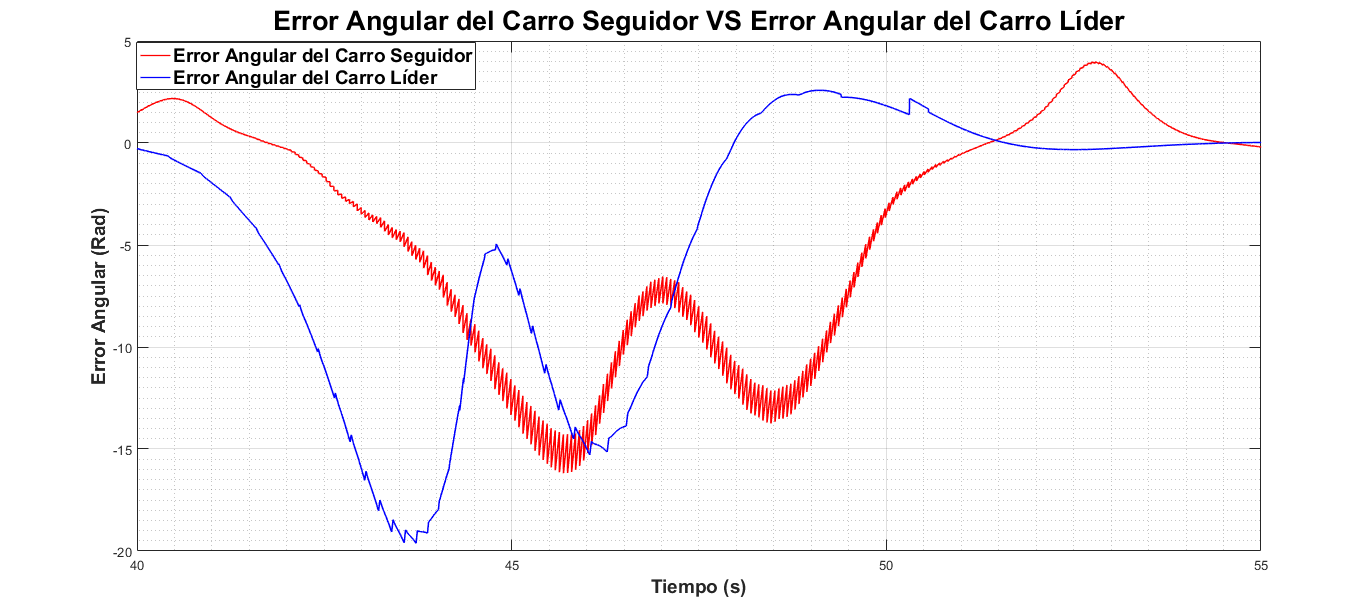
\includegraphics[scale=0.35]{Imagenes/csea}
		\caption{Gráfica del error angular de los vehículos}
		\label{fig:csea}
\end{figure}	

\begin{figure}[H]
	\centering
		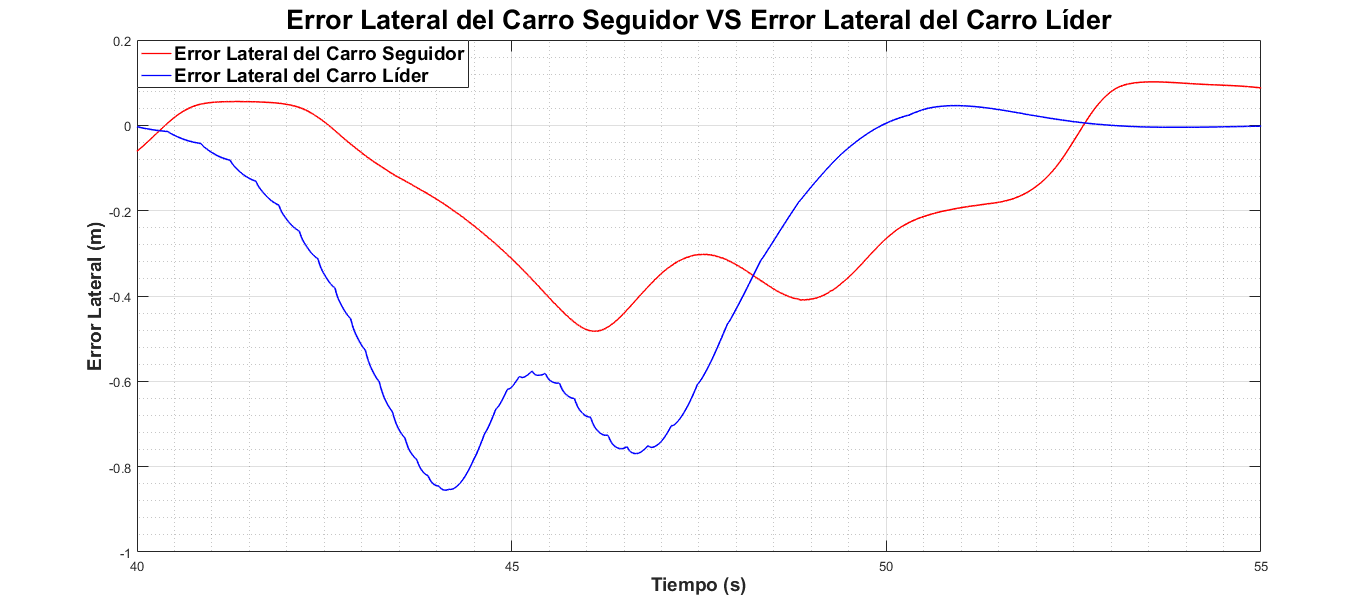
\includegraphics[scale=0.35]{Imagenes/csel}
		\caption{Gráfica del error lateral de los vehículos}
		\label{fig:csel}
\end{figure}	

%\begin{figure}[H]
%	\centering
%		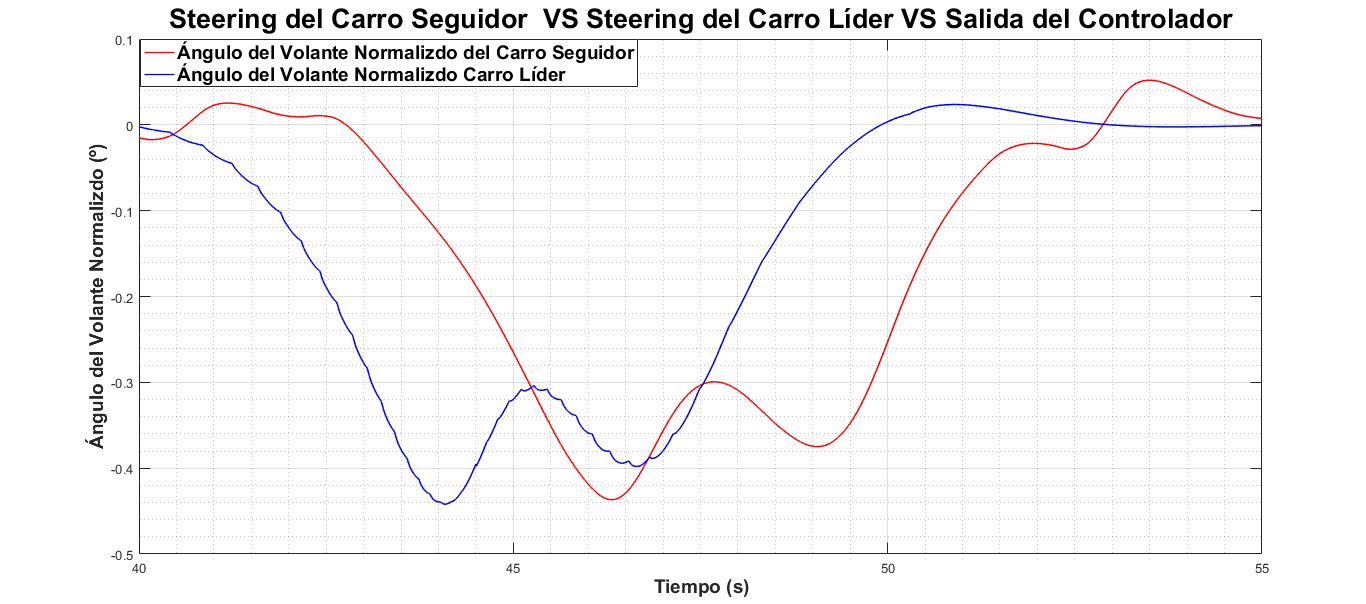
\includegraphics[scale=0.35]{Imagenes/csst}
%		\caption{Gráfica del ángulo del volane de los vehículos}
%		\label{fig:csst}
%\end{figure}	


%%%%%%%%%%%%%%%%%%%%%%%%%%%%%%%%%%%%
\section{\textit{Stop and Go}}
%%%%%%%%%%%%%%%%%%%%%%%%%%%%%%%%%%%%
En esta maniobra se busca evaluar la capacidad del vehículo para frenar en caso de que se presente algun improvisto, más específicamente, cuando el vehículo que tiene al frente realiza un frenado brusco. Para realizar esta maniobra, se emplea el mismo controlador desarrollado para el ACC, siguiendo de esta forma, el mismo principio, mantener la misma velocidad, con una cierta distancia de seguridad.

%%%%%%%%%%%%%%%%%%%%%%%%%%%%
\subsection{Pruebas en Dynacar a Distintas Velocidades}
%%%%%%%%%%%%%%%%%%%%%%%%%%%%
Para evaluar el desempeño del controlador en esta maniobra se realizaron cuatro purebas, donde se aceleraba hasta cierto punto y luego de un tiempo se frenaba rápidamente, estas pruebas se dividen en dos grupos, las de velocidad baja y las de velocidad media.  
 
%%%%%%%%%%%%%%%%%%%%%%%
\subsubsection{Velocidades Bajas}
%%%%%%%%%%%%%%%%%%%%%%%
A continuación se presentan las gráficas de velocidad y distancia, cuando se alcanzan velocidades de 10 Km/h y 20 Km/h. 
\begin{itemize}

\item 10 Km/h:

Observando la Figura \ref{fig:velstg10} se aprecia que el vehículo seguidor mantiene en todo momento la velocidad de referencia , y al instante de realizar el frenado, lo hace al mismo tiempo. En el caso de la distancia, en la Figura \ref{fig:diststg10} se contempla que después de realizar el frenado el vehículo queda a una distancia de 6,8 m, presentando así, un error del 3 \%, valor aceptable, ya que se encuentra a una buena distancia, que garantiza seguridad en la maniobra.\\
 
\begin{figure}[H]
	\centering
		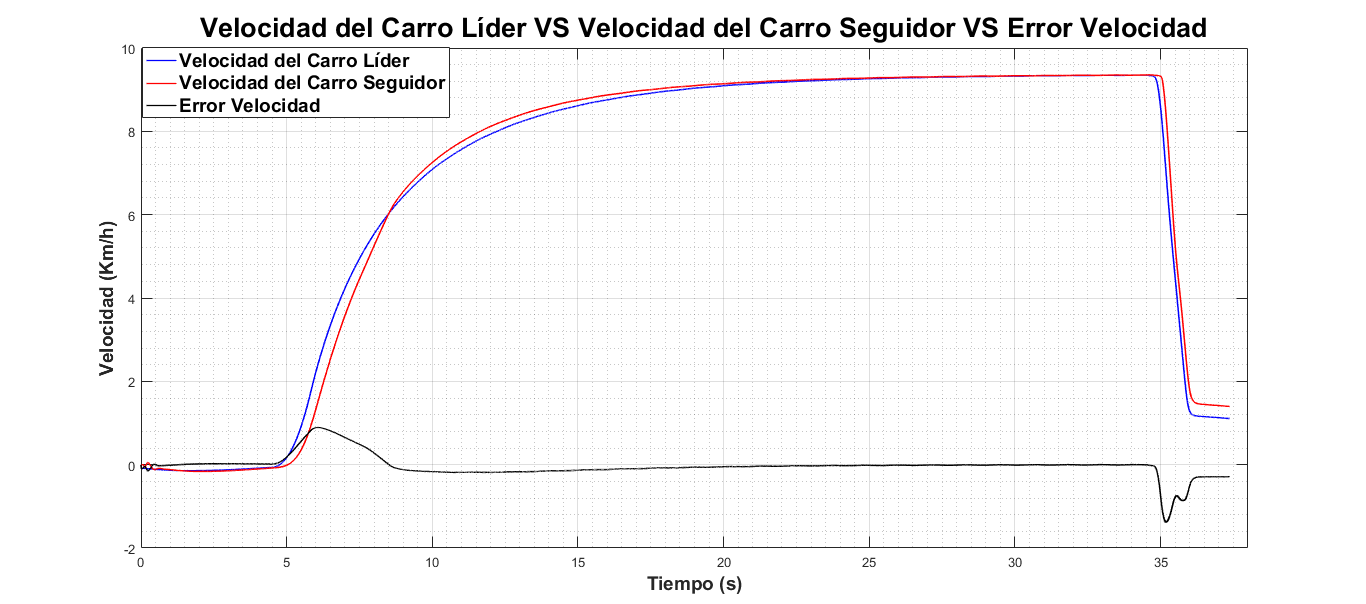
\includegraphics[scale=0.35]{Imagenes/stg10}
		\caption{Gráfica de la velocidad de los vehículos}
		\label{fig:velstg10}
\end{figure}	

\begin{figure}[H]
	\centering
		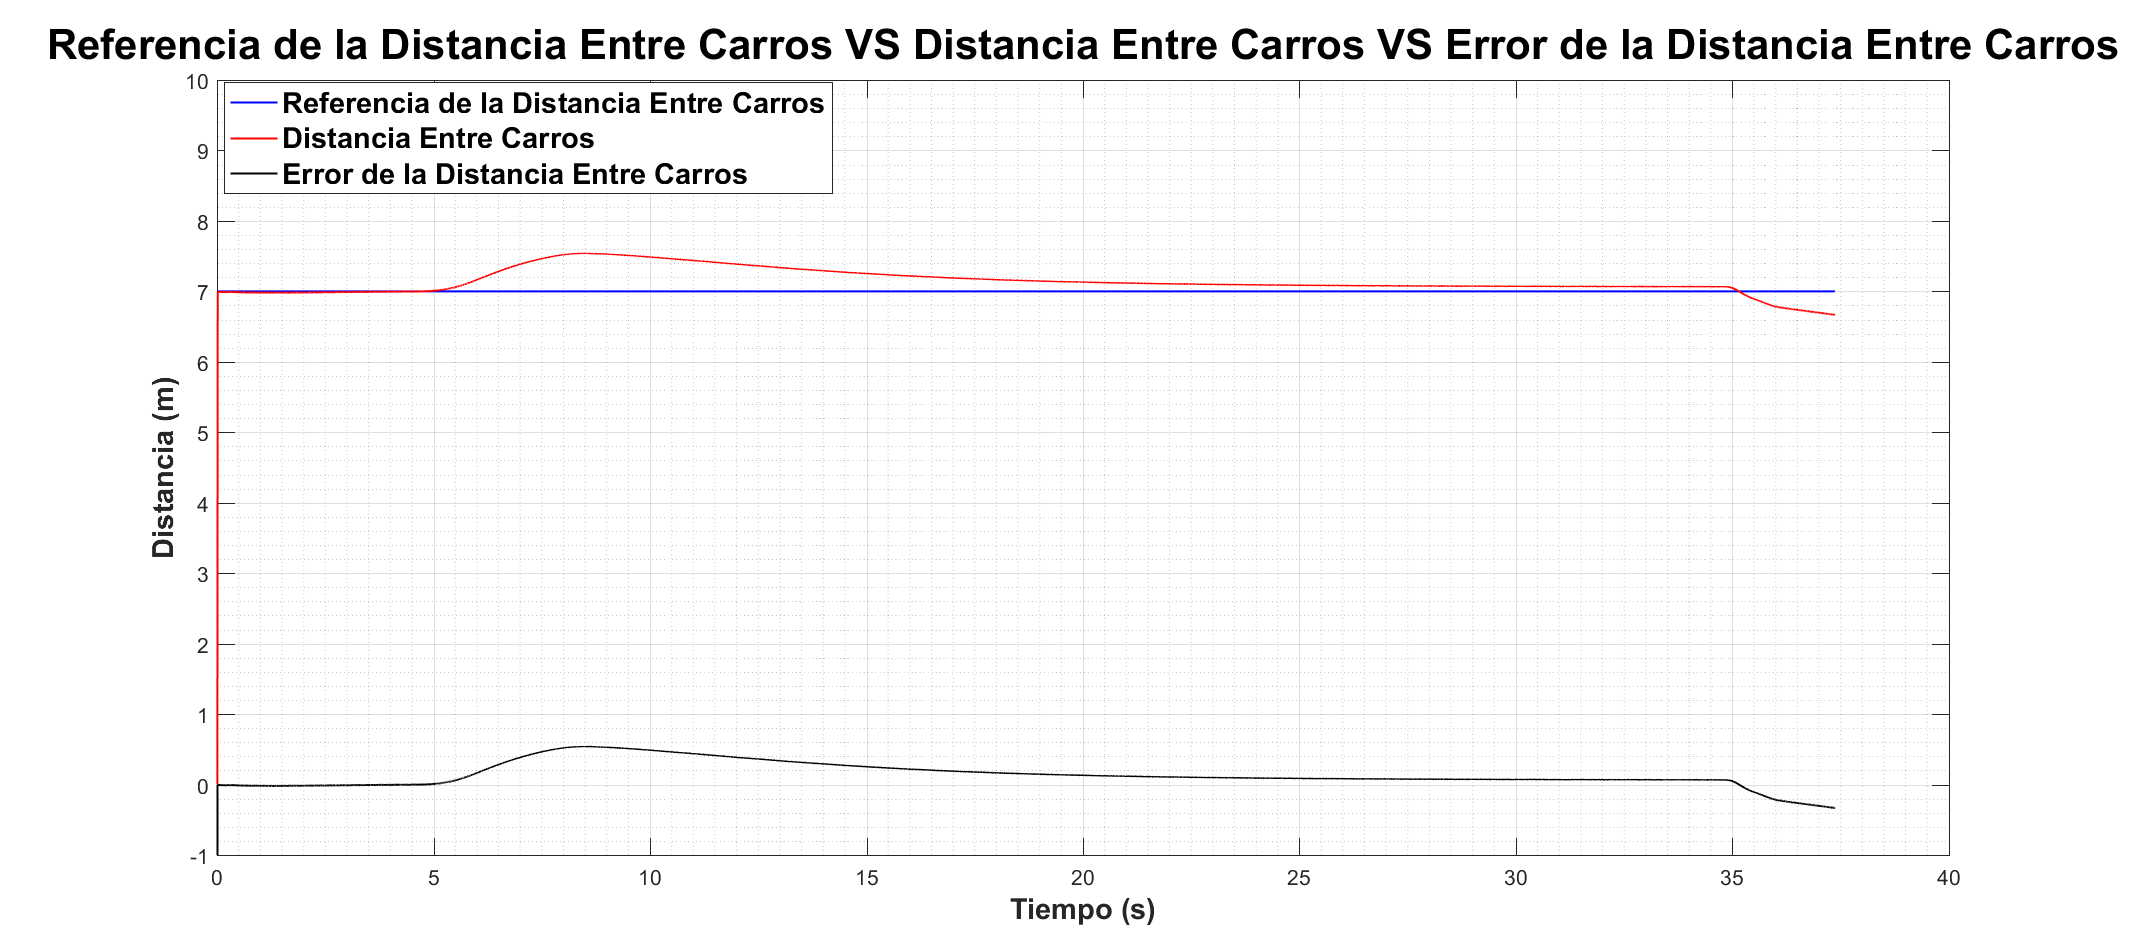
\includegraphics[scale=0.35]{Imagenes/stg10dist}
		\caption{Gráfica del error de la distancia de los vehículos}
		\label{fig:diststg10}
\end{figure}	

\item 20 Km/h:

En la Figura \ref{fig:velstg20} se aprecia que el vehículo supera la velocidad del vehículo líder hasta alcanzar la distancia de referencia, posteriormente se observa como carro comienza a frenar a la par que el carro líder, y se mantiene así, hasta el punto donde cambia el valor de referencia de la distancia, prodicendo que el frenado tarde un poco más en hacerse. Estos cambios de distancias, pueden ser vistos en la Figura \ref{fig:diststg20}, en la cual, además se contempla que después de realizar el frenado el vehículo queda a una distancia de 6,6 m, presentando así, un error del 5 \%.

\begin{figure}[H]
	\centering
		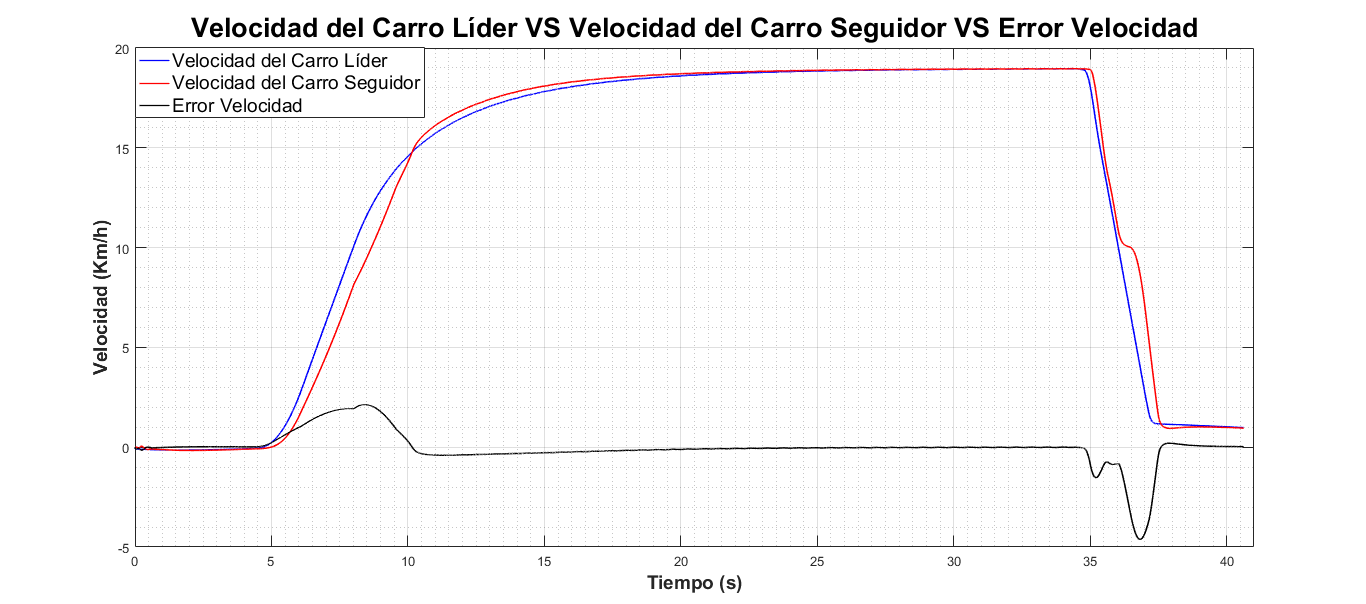
\includegraphics[scale=0.35]{Imagenes/stg20}
		\caption{Gráfica de la velocidad de los vehículos}
		\label{fig:velstg20}
\end{figure}	

\begin{figure}[H]
	\centering
		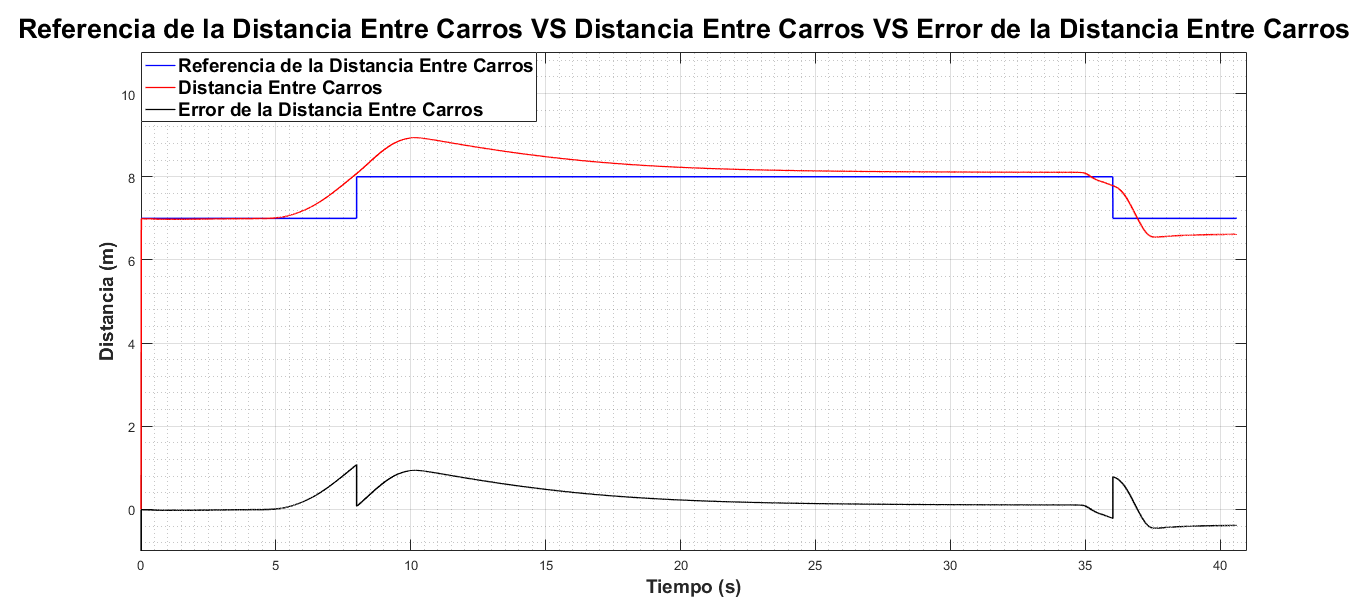
\includegraphics[scale=0.35]{Imagenes/stg20dist}
		\caption{Gráfica del error de la distancia de los vehículos}
		\label{fig:diststg20}
\end{figure}	

\end{itemize}
%%%%%%%%%%%%%%%%%%%%%%%
\subsubsection{Velocidades Medias}
%%%%%%%%%%%%%%%%%%%%%%%
A continuación se presentan las gráficas de velocidad y distancia, cuando se alcanzan velocidades de 40 Km/h y 50 Km/h. 

\begin{itemize}

\item 40 Km/h:

Como se puede observar en la Figura \ref{fig:velstg40}, el frenado del vehículo seguidor no es realizado de forma brusca, sino progresivo, esto, con el fin de reducir los efectos que pueda tener el frenado repentino, sobre el conductor. Además, en la Figura\ref{fig:diststg40} se aprecia que el vehículo logra frenar, guardando completamente la distancia de seguridad.\\
   
\begin{figure}[H]
	\centering
		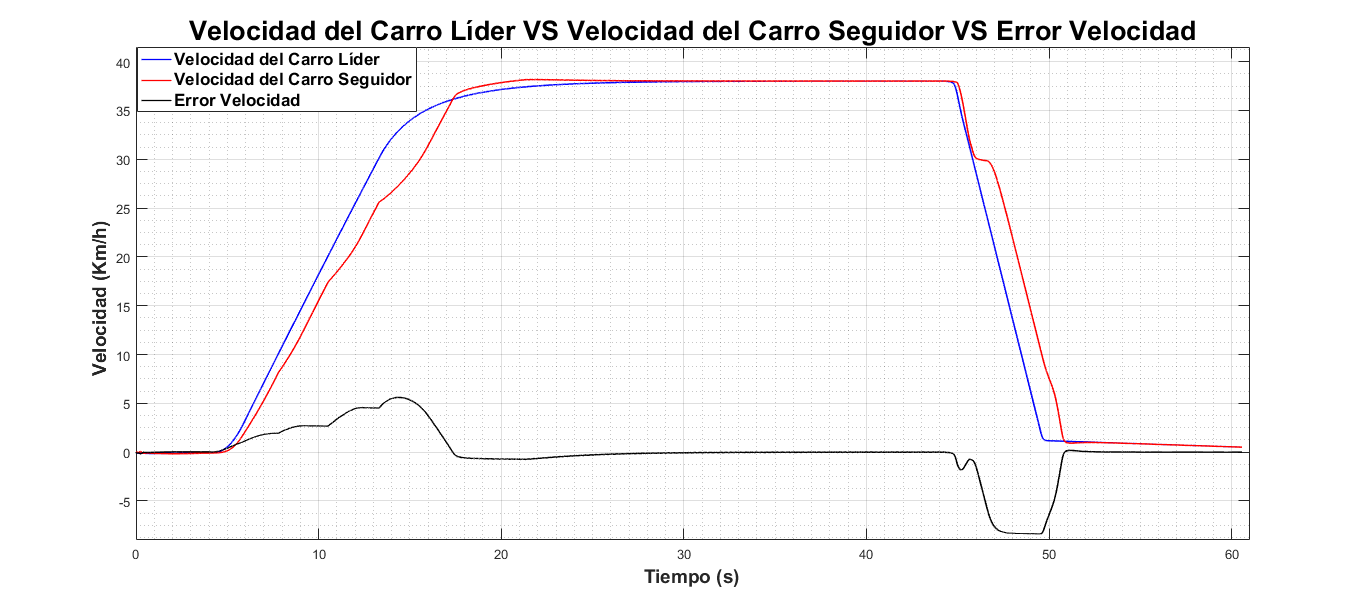
\includegraphics[scale=0.35]{Imagenes/stg40}
		\caption{Gráfica de la velocidad de los vehículos}
		\label{fig:velstg40}
\end{figure}	

\begin{figure}[H]
	\centering
		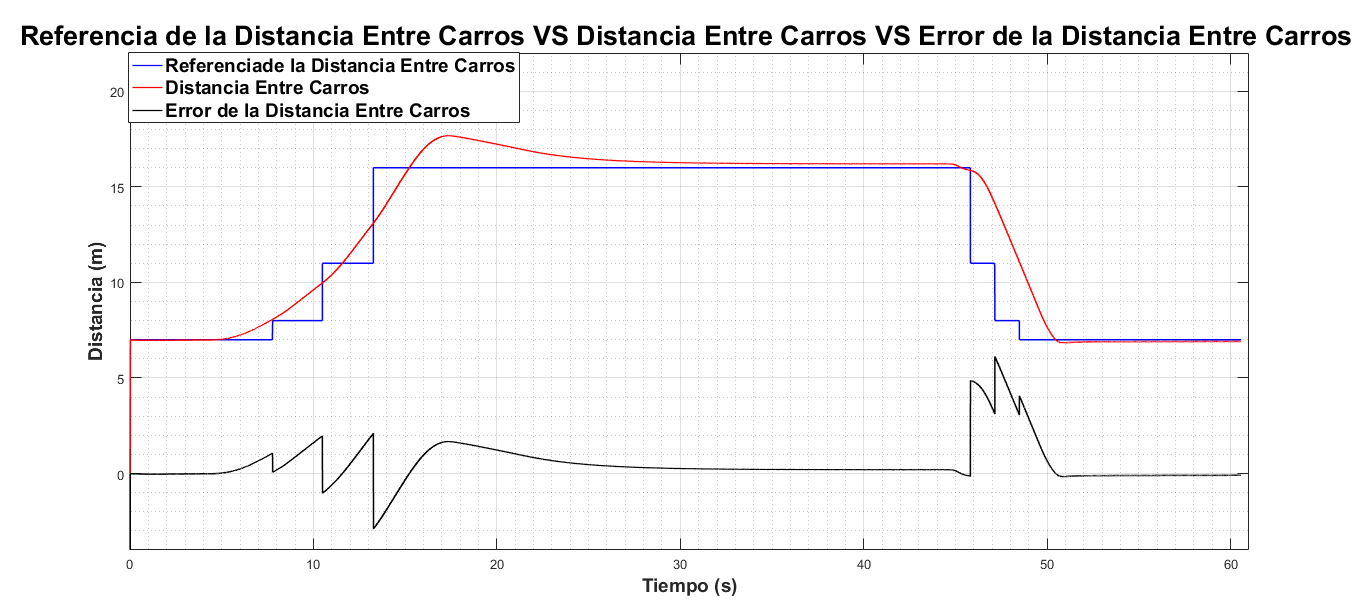
\includegraphics[scale=0.35]{Imagenes/stg40dist}
		\caption{Gráfica del error de la distancia de los vehículos}
		\label{fig:diststg40}
\end{figure}	

%%%%%%%%%%%%%%%%%%%%%%%
\item50 Km/h:
%%%%%%%%%%%%%%%%%%%%%%%

Como se puede observar en la Figura \ref{fig:velstg50}, de igual forma el frenado del vehículo seguidor es realizado de una forma más progresiva, con la diferencia de que para alcanzar el valor de referencia de la distancia, se tuvo que sobrepasar en buena media la velocidad del vehículo líder. No obstante, se puede apreciar que en la Figura\ref{fig:diststg50} el vehículo logra frenar, guardando completamente la distancia de seguridad.\\

\begin{figure}[H]
	\centering
		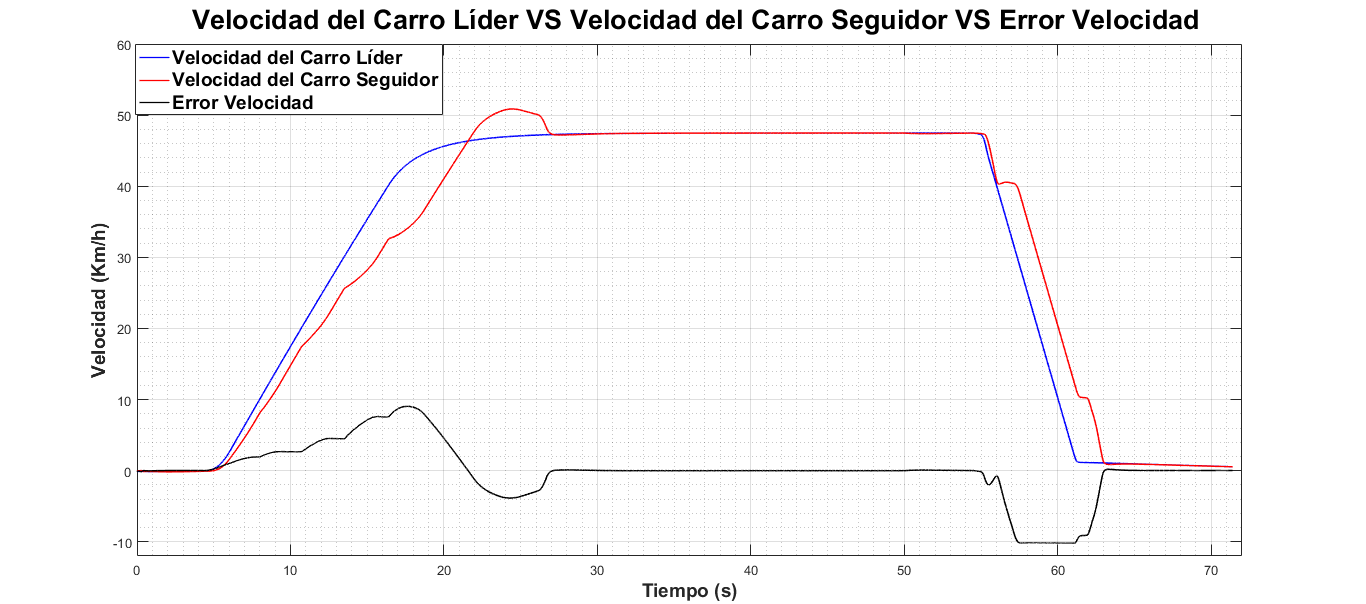
\includegraphics[scale=0.35]{Imagenes/stg50}
		\caption{Gráfica de la velocidad de los vehículos}
		\label{fig:velstg50}
\end{figure}	

\begin{figure}[H]
	\centering
		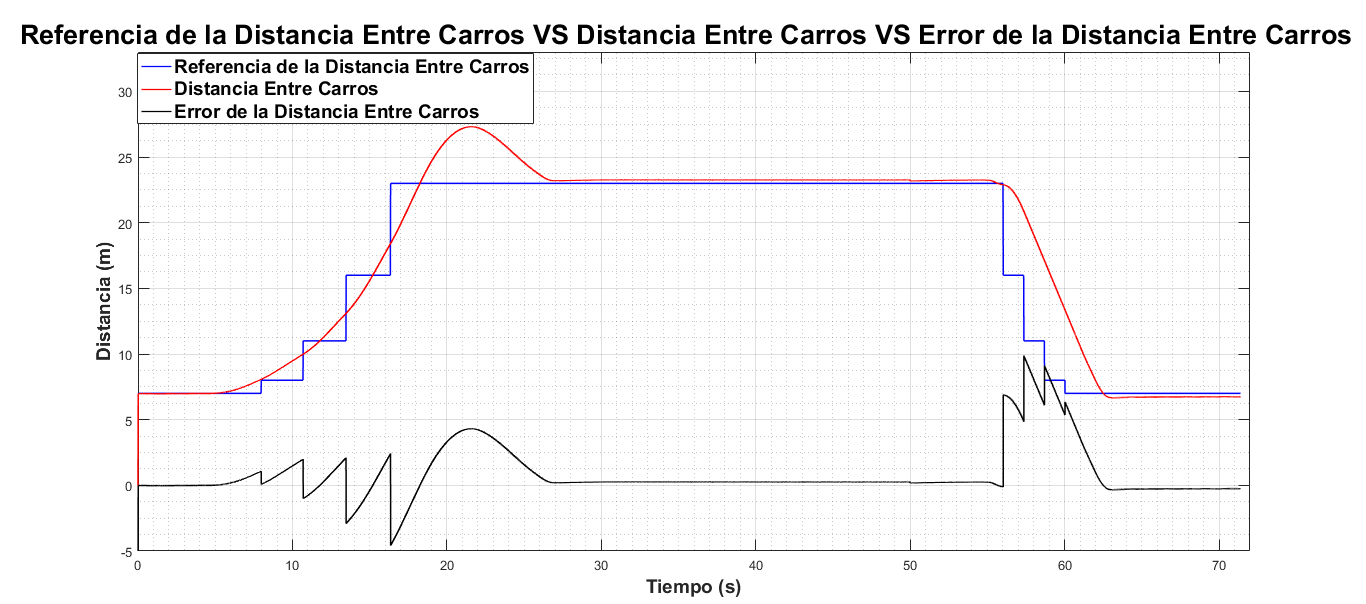
\includegraphics[scale=0.35]{Imagenes/stg50dist}
		\caption{Gráfica del error de la distancia de los vehículos}
		\label{fig:diststg50}
\end{figure}	
\end{itemize}

%%%%%%%%%%%%%%%%%%%%%%%%%%%%%%%%%%%%%%%
\section{ACC Longitudinal con Control Lateral}
%%%%%%%%%%%%%%%%%%%%%%%%%%%%%%%%%%%%%%%

En esta maniobra se prueba el rendimiento de ambos controladores juntos, permitiendo el seguimiento completamente autónomo de un vehículo, es decir, que pueda maneter la misma velocidad que el vehículo que tenga al frente, así como una distancia de margen, además de poder seguir la ruta que plantea dicho vehículo. De la igual forma que de las demás pruebas, la misma se realizó empleando dos modelos de Dynacar en Simulink.
  
\subsection{Pruebas en Dynacar con Distintos Tipos de Curvas Variando la Velocidad}

Las pruebas realizadas se hicieron de la misma forma que para el Control Lateral solo, es decir en el escenario de la pista de TECNALIA \textit{Research \& Innovation} (Figura \ref{fig:tecnaliap2}), la cual se dividió en los mismo tres segmentos, cambio de carril, curva fuerte y curva suave. En dichos tramos, se observa como se ven influenciados ambos controladores, al funcionar juntos. 

%%%%%%%%%%%%%%%%%%%%%%%
\subsubsection{Cambio de Carril}
%%%%%%%%%%%%%%%%%%%%%%%

Correspondiente al segundo tramo, las Figuras \ref{fig:vacc} y \ref{fig:distcc}, muestra el comportamiento del ACC, tanto de velocidad como de distancia. Pudiéndose apreciar, un buen comportamiento, apegándose a las referencias, aún existiendo cambios de velocidad.\\

\begin{figure}[!h]
	\centering
		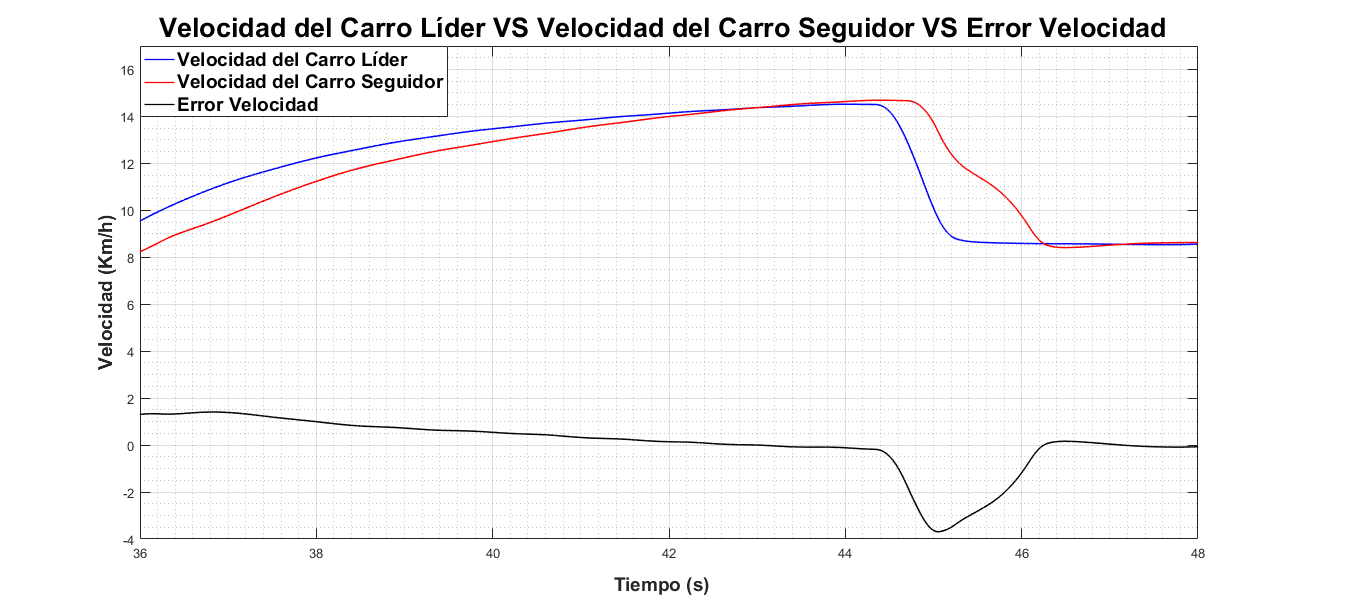
\includegraphics[scale=0.35]{Imagenes/vacc}
		\caption{Gráfica de la velocidad de los vehículos}
		\label{fig:vacc}
\end{figure}	 

\begin{figure}[!h]
	\centering
		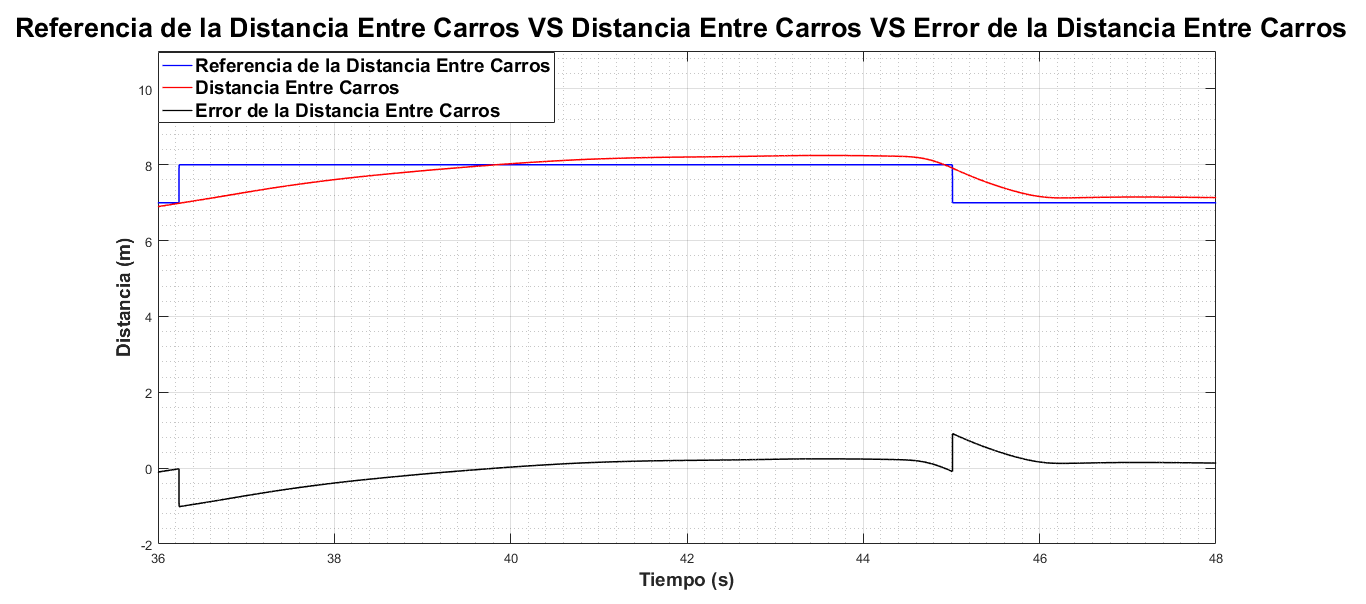
\includegraphics[scale=0.35]{Imagenes/dacs}
		\caption{Gráfica del error de la distancia de los vehículos}
		\label{fig:distcc}
\end{figure}	 

 %\begin{figure}[H]
 %\centering
  %\subfloat[Gráfica de la velocidad de los vehículos]{
   %\label{fig:velcc}
    %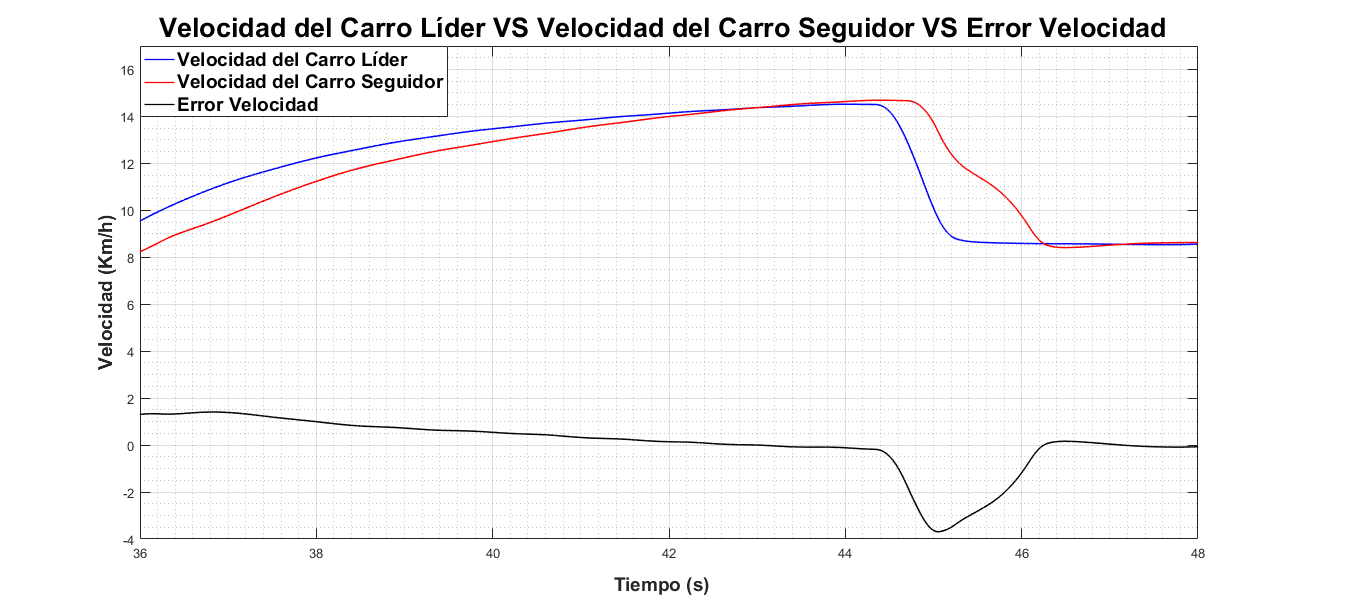
\includegraphics[scale=0.28]{Imagenes/vacc}}\\
  %\subfloat[Gráfica del error de la distancia de los vehículos]{
   %\label{fig:distcc}
   % 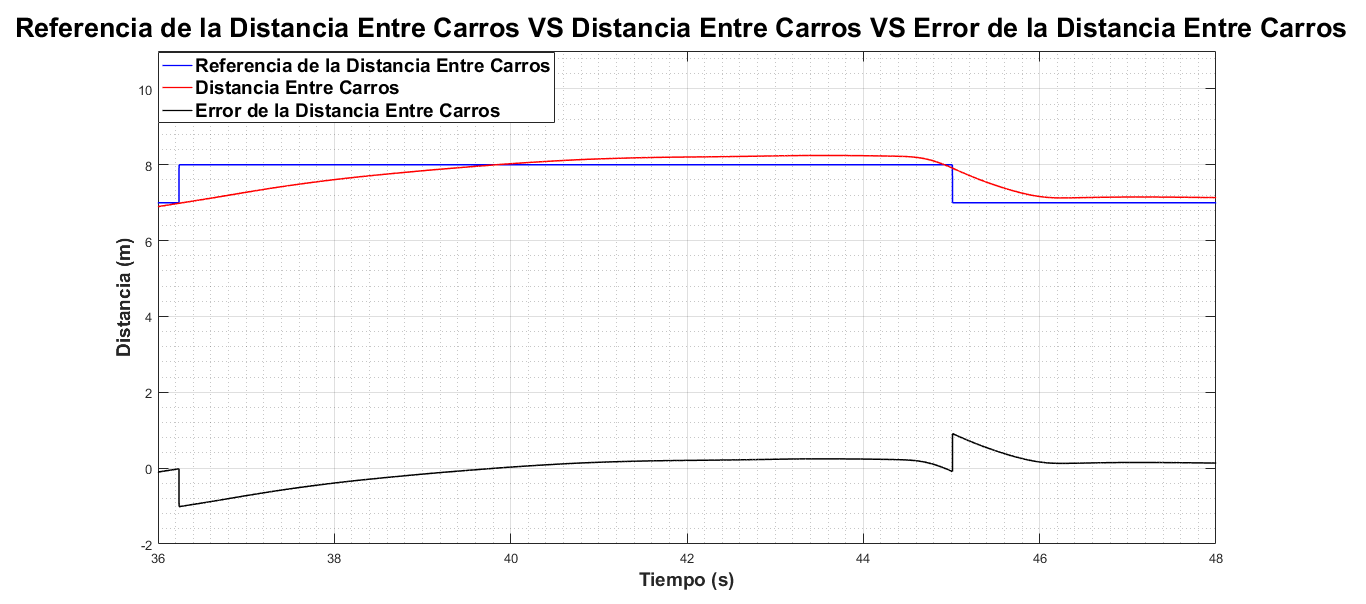
\includegraphics[scale=0.28]{Imagenes/dacs}}
 %\caption{Comportamiento del ACC en un cambio de carril}
 %\label{fig:acccc}
%\end{figure}

\par En cuanto a la ruta seguida (Figura \ref{fig:arcc}) se puede apreciar que, al igual que la Figura \ref{fig:rcc}, ambos vehículos poseen una trayectoria similar a la del planificador local, viéndose diferensiado un poco a la hora de realizar la acción, momento que a su vez coincide con el cambio de velocidad. 

\begin{figure}[H]
 \centering
  \subfloat[Gráfica de la ruta seguida por los vehículos]{
   \label{fig:avcc}
    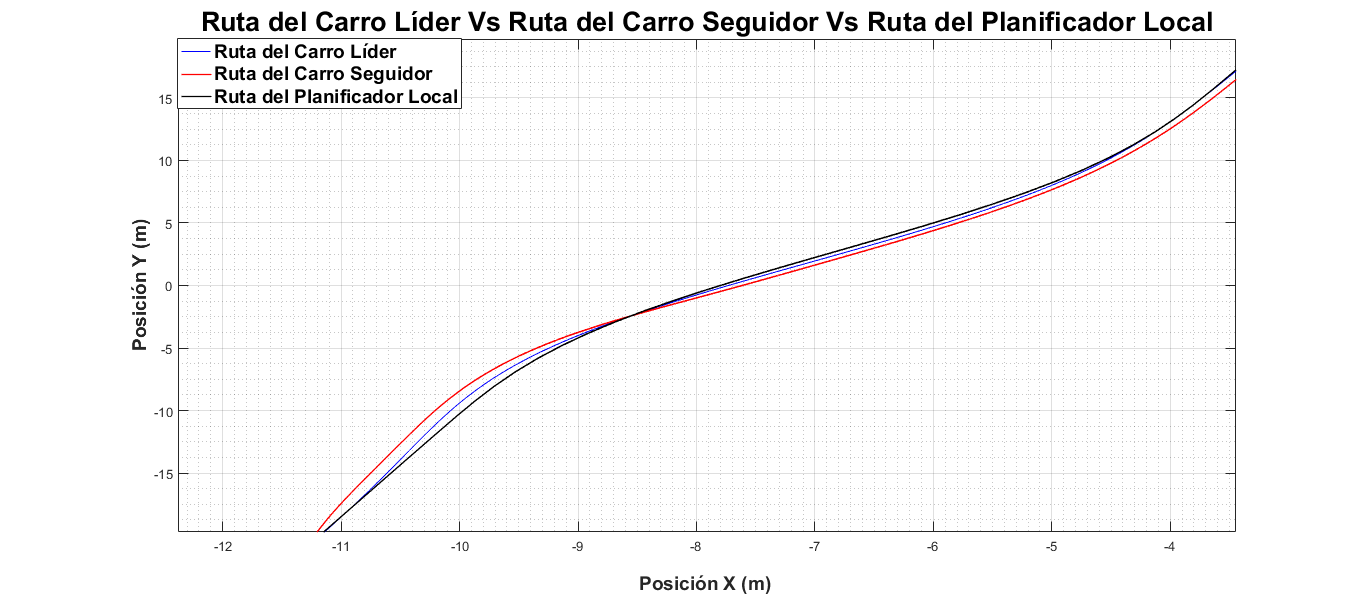
\includegraphics[scale=0.27]{Imagenes/arcc}}
  \subfloat[Ruta seguida por los vehículos en Dynacar]{
   \label{fig:adcc}
    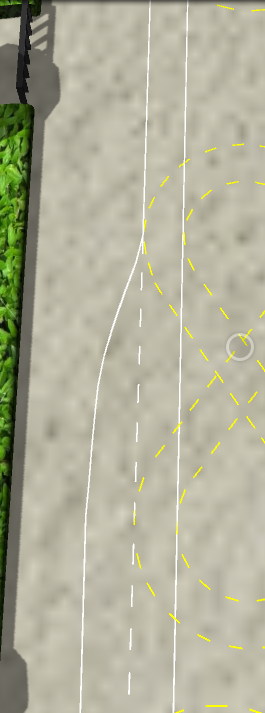
\includegraphics[scale=0.27]{Imagenes/dcf}}
 \caption{Ruta establecida para el cambio de carril}
 \label{fig:arcc}
\end{figure}

\par En las Figuras \ref{fig:aerang} y \ref{fig:aerlat}, se pueden encontrar los errores lateral y angular de ambos vehículos, teniendo que para el vehículo seguidor, el error angular es de 5.5 grados, y el lateral de unos 15.2 cm, valores muy similares a los obtenidos con el Control Lateral solo, mientras que para el carro líder no se presenta ningún cambio, con lo cual, niguno de los dos controladores vieron afectado sus desempeños en esta acción.

\begin{figure}[H]
	\centering
		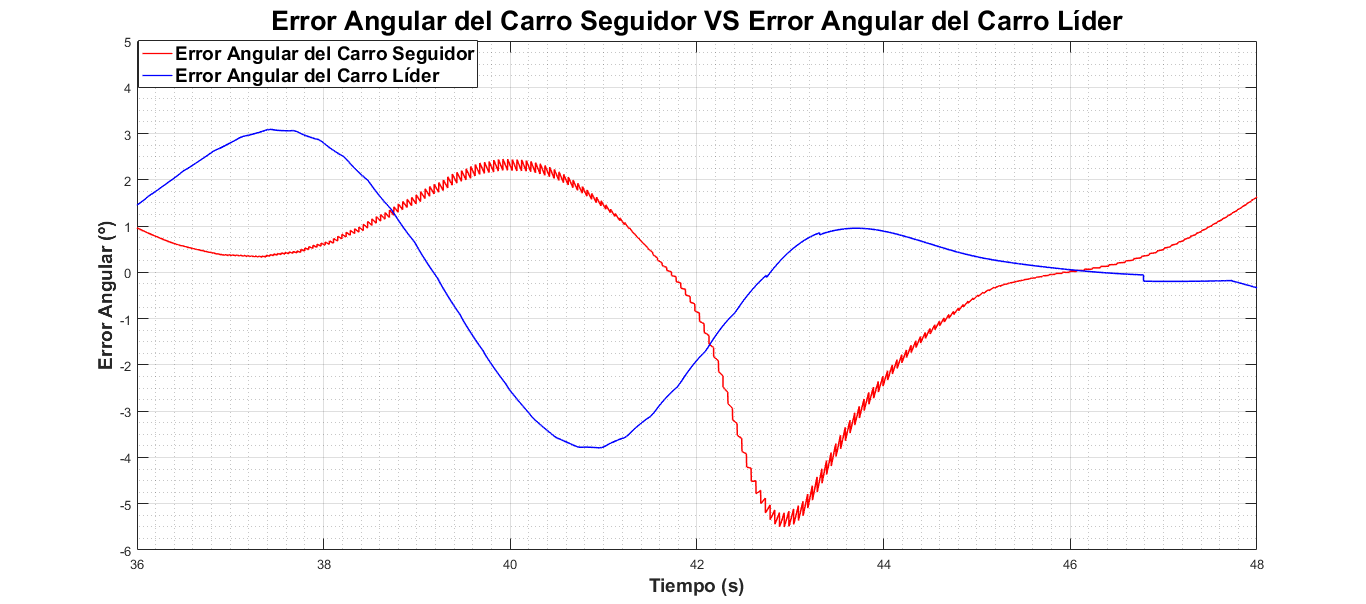
\includegraphics[scale=0.34]{Imagenes/accea}
		\caption{Gráfica del error angular de los vehículos}
		\label{fig:aerang}
\end{figure}	

\begin{figure}[H]
	\centering
		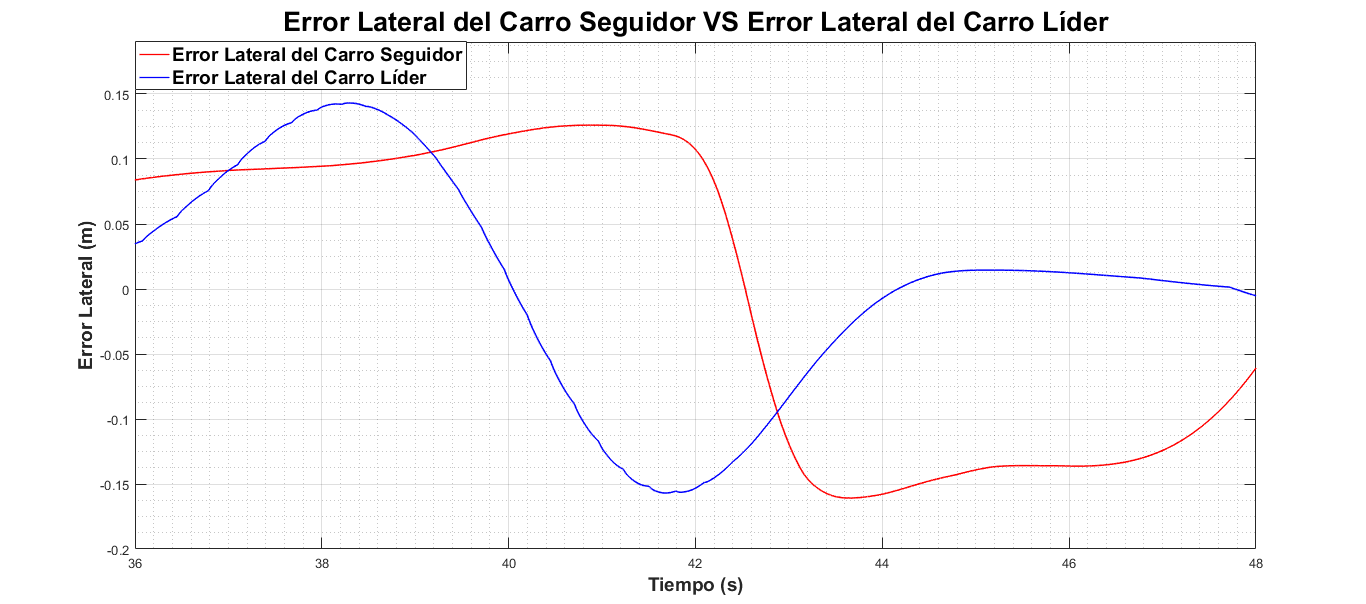
\includegraphics[scale=0.35]{Imagenes/accel}
		\caption{Gráfica del error lateral de los vehículos}
		\label{fig:aerlat}
\end{figure}	

%\begin{figure}[H]
%	\centering
%		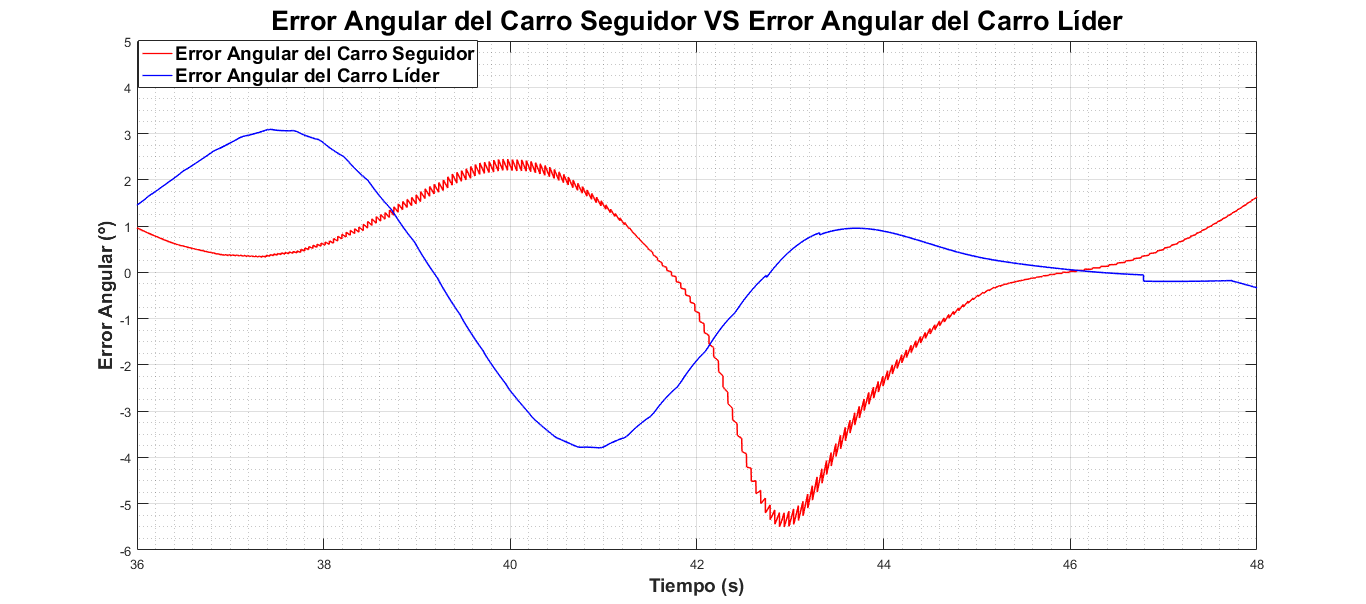
\includegraphics[scale=0.35]{Imagenes/accea}
%		\caption{Gráfica del ángulo del volante de los vehículos}
%		\label{fig:aerst}
%\end{figure}	


%%%%%%%%%%%%%%%%%%%%%%%
\subsubsection{Curvas}
%%%%%%%%%%%%%%%%%%%%%%%
A continuación, se presenta la curva correspondiente al primer tramo, la cual posee una curvatura más pronunciada. En este trayecto se obtuvo que, el controlador (Figuras \ref{fig:aervel} y \ref{fig:aerdist}) mostró un buen desempeño, a pesar de ver aumentado su error al estabilizarce, en el momento de pasar por la curva, siendo estos, 0.1 Km/h, para la velocidad y 50 cm, para la distancia, valores que de igual forma, pueden ser despreciados. \\

\begin{figure}[H]
	\centering
		\includegraphics[scale=0.35]{Imagenes/vacf}
		\caption{Gráfica de las velocidades de los vehículos}
		\label{fig:aervel}
\end{figure}	

\begin{figure}[H]
	\centering
		\includegraphics[scale=0.35]{Imagenes/dacf}
		\caption{Gráfica del error de distancia de los vehículos}
		\label{fig:aerdist}
\end{figure}	

\par En este caso la ruta seguida por ambos vehículos, posee la misma forma que la de la Figura \ref{fig:rcf}, un mayor error en el tramo final de la curva, con respecto a la generada por el planificador local, pero con una similitud peuqeña entre ellas. De igual forma ambos vehículos se encuentran dentro de los límites del carril donde circulan.\\

\begin{figure}[H]
 \centering
  \subfloat[Gráfica de la ruta seguida por los vehículos]{
   \label{fig:a}
    \includegraphics[scale=0.28]{Imagenes/arcf}}
  \subfloat[Ruta seguida por los vehículos en Dynacar]{
   \label{fig:v}
    \includegraphics[scale=0.28]{Imagenes/dcc}}
 \caption{Ruta establecida para la curva fuerte}
 \label{fig:rec}
\end{figure}

\par En lo que respecta a los errores, las Figuras \ref{fig:acfea} y \ref{fig:acfel} muestran que los mismos poseen un valor máximo de, 19 grados y 0.44 m, siendo ligeramente menores a los presentados por el Control Lateral solo, efecto que se debe a que, en el momento de realizar la acción la velocidad del vehículo seguidor era menor, que la fijada en la otra prueba.\\ 
 
\begin{figure}[H]
	\centering
		\includegraphics[scale=0.35]{Imagenes/acfea}
		\caption{Gráfica del error angular de los vehículos}
		\label{fig:acfea}
\end{figure}	

\begin{figure}[H]
	\centering
		\includegraphics[scale=0.35]{Imagenes/acfel}
		\caption{Gráfica del error lateral de los vehículos}
		\label{fig:acfel}
\end{figure}	

%\begin{figure}[H]
%	\centering
%		\includegraphics[scale=0.35]{Imagenes/acfst}
%		\caption{Gráfica del ángulo del volane de los vehículos}
%		\label{fig:acfst}
%\end{figure}	

\par En el caso de la segunda curva, la cual corresponde al tercer segmento, se tiene que la velocidad (Figura \ref{fig:acvelcs}), permance constante y  sin ninguna alteración, durante la curva, mientras que en la distancia (Figura \ref{fig:acdistcs}) se presenta un pequeño error de 30 cm, equivalente al 4 \% , error que de igual forma puede ser considerado como despreciable.\\

\begin{figure}[H]
	\centering
		\includegraphics[scale=0.35]{Imagenes/vacs}
		\caption{Gráfica de la velocidad de los vehículos}
		\label{fig:acvelcs}
\end{figure}	

\begin{figure}[H]
	\centering
		\includegraphics[scale=0.35]{Imagenes/dacc}
		\caption{Gráfica del error de la distancia de los vehículos}
		\label{fig:acdistcs}
\end{figure}	


\par En cuanto a la ruta seguida por los vehículos (Figura \ref{fig:arcs}) se observa, que posee la misma forma que la seguida por los vehículos con solo el Control Lateral, es decir, separadas en una pequeña medida de la ruta del plainifcador local, pero prácticamente igual una a la otra.\\  

\begin{figure}[H]
 \centering
  \subfloat[Gráfica de la ruta seguida por los vehículos]{
   \label{fig:avcs}
    \includegraphics[scale=0.28]{Imagenes/racs}}
  \subfloat[Ruta seguida por los vehículos en Dynacar]{
   \label{fig:adcs}
    \includegraphics[scale=0.28]{Imagenes/dcs}}
 \caption{Ruta establecida para una curva suave}
 \label{fig:arcs}
\end{figure}

\par Esta similitud en la ruta, se puede ver comprobada con las Figuras \ref{fig:acsea} y \ref{fig:acsel}, las cuales muestran que los errores angulares y laterales máximos, del vehículo seguidor son de 15 grados y 41 cm, iguales a los presentados por el Control Lateral solo, observandoo de esta forma que no se ve afectado por el cambio de velocidades producido por el ACC.\\

\begin{figure}[H]
	\centering
		\includegraphics[scale=0.35]{Imagenes/acsea}
		\caption{Gráfica del error angular de los vehículos}
		\label{fig:acsea}
\end{figure}	

\begin{figure}[H]
	\centering
		\includegraphics[scale=0.35]{Imagenes/acsel}
		\caption{Gráfica del error angular de los vehículos}
		\label{fig:acsel}
\end{figure}	

%\begin{figure}[H]
%	\centering
%		\includegraphics[scale=0.35]{Imagenes/acsst}
%		\caption{Gráfica del ángulo del volane de los vehículos}
%		\label{fig:acsst}
%\end{figure}	

\section{Resumen}

En el presente capítulo se presentaron los algoritmos e implementación de los contralores empleados para efectuar las maniobras, seguidamente se mostraron los resultados de las pruebas de dichas maniobras, sin la utilización de comunicaciones vehiculares, empleando la herramienta de Simulink que permite introducir dos bloques de Dynacar en un mismo esquema.\\

\par  Dentro de los resultados obtenidos se destaca, el correcto comportamiento del controlador para el ACC, el cual mostró un bajo error para esta maniobra, tanto para velocidades bajas, como medias, de igual forma que para la maniobra de \textit{Stop and Go}. Además también se puede resaltar el buen desempeño del Control Lateral, al utilizarse individualmente y en conjunto con la maniobra de ACC.